\documentclass[a4paper]{article}

\usepackage[top=1.5cm, right=2cm, bottom=1.5cm, left=2cm]{geometry}
\usepackage{amsmath, amsfonts, amssymb}
\usepackage[utf8]{inputenc}
\usepackage[T1]{fontenc}
\usepackage[brazilian]{babel}
\usepackage{xcolor}

\usepackage{graphicx}
\usepackage{float}
\usepackage{pdfpages}
\usepackage{hyperref}

\begin{document}
	
\includepdf[pages={1}]{titlepage}
	\section{Composição padrão}
	\begin{figure}[ht!]
		\hspace{-7.7cm}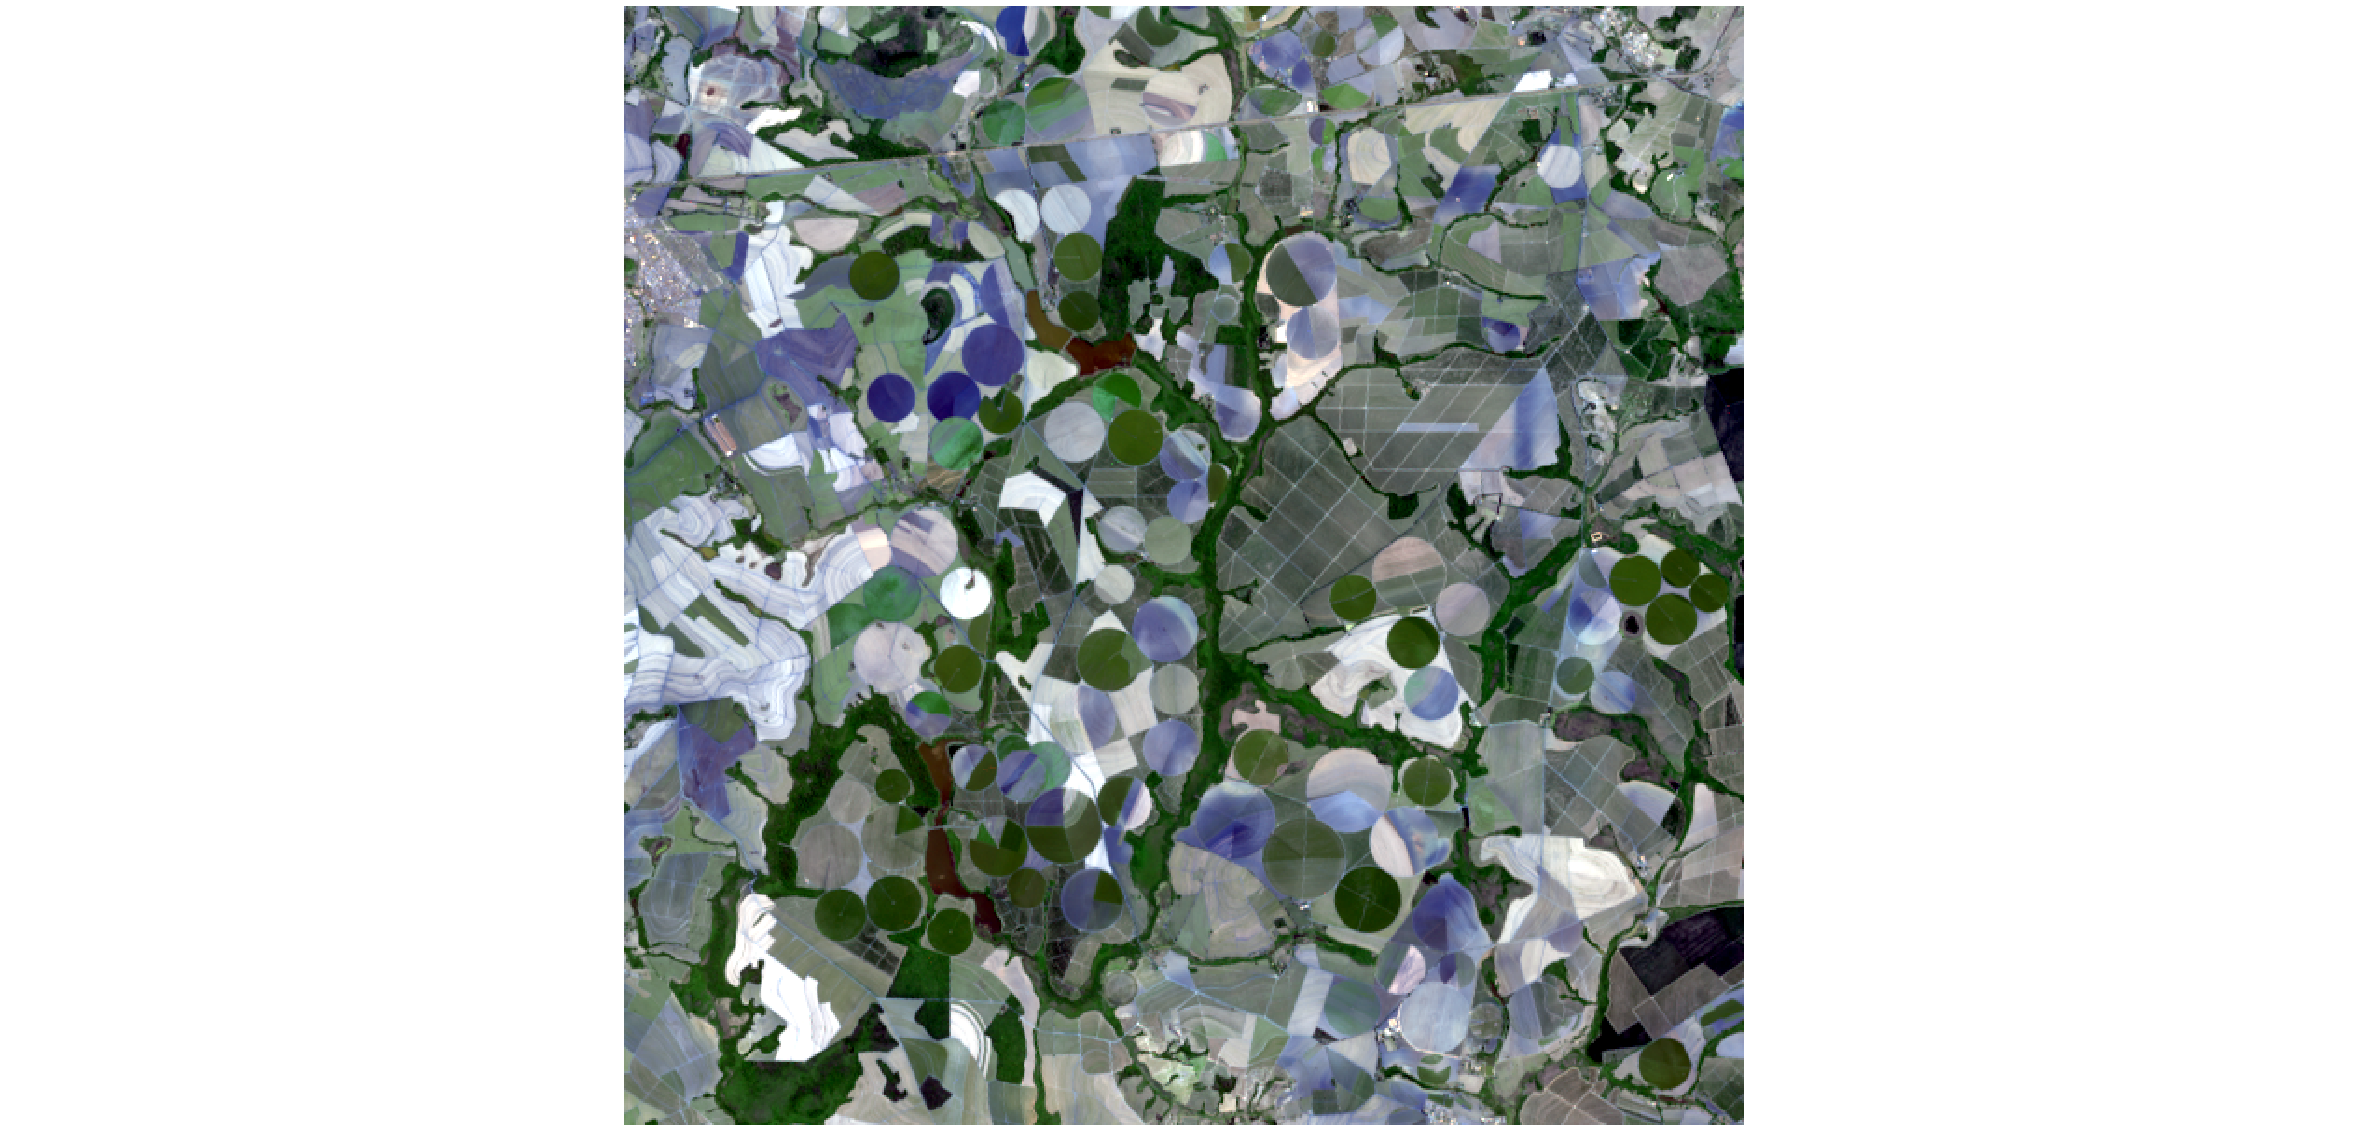
\includegraphics[width=1.9\linewidth]{../images/default}
		\caption{Composição padrão na importação do banco de dados no RGB234}
	\end{figure}
	\section{Composições coloridas}
	\begin{figure}[H]
		\centering
		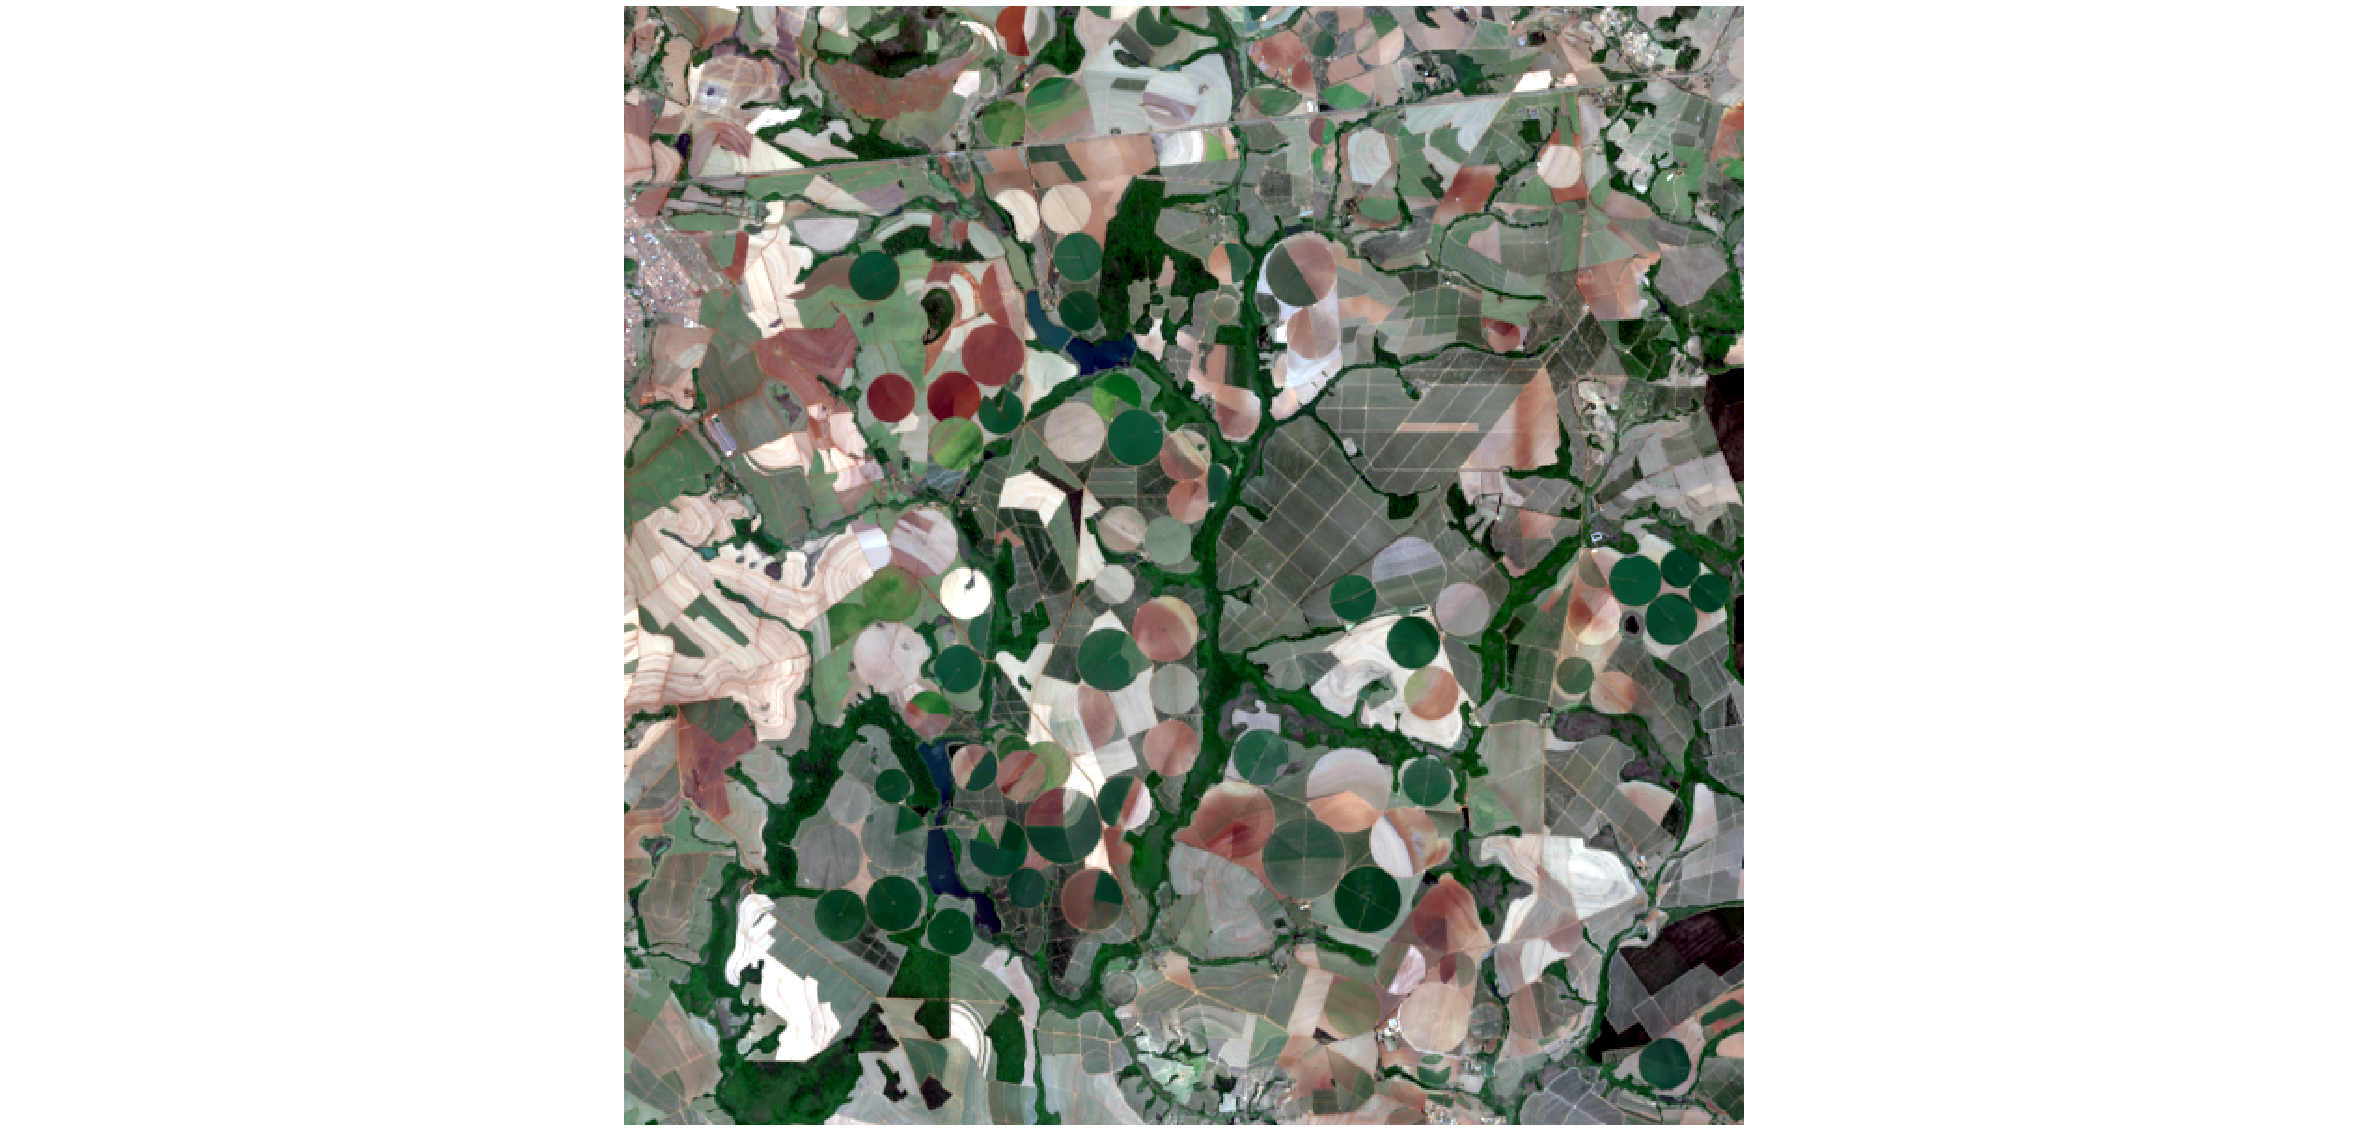
\includegraphics[width=1.\linewidth]{../images/rgb432}
		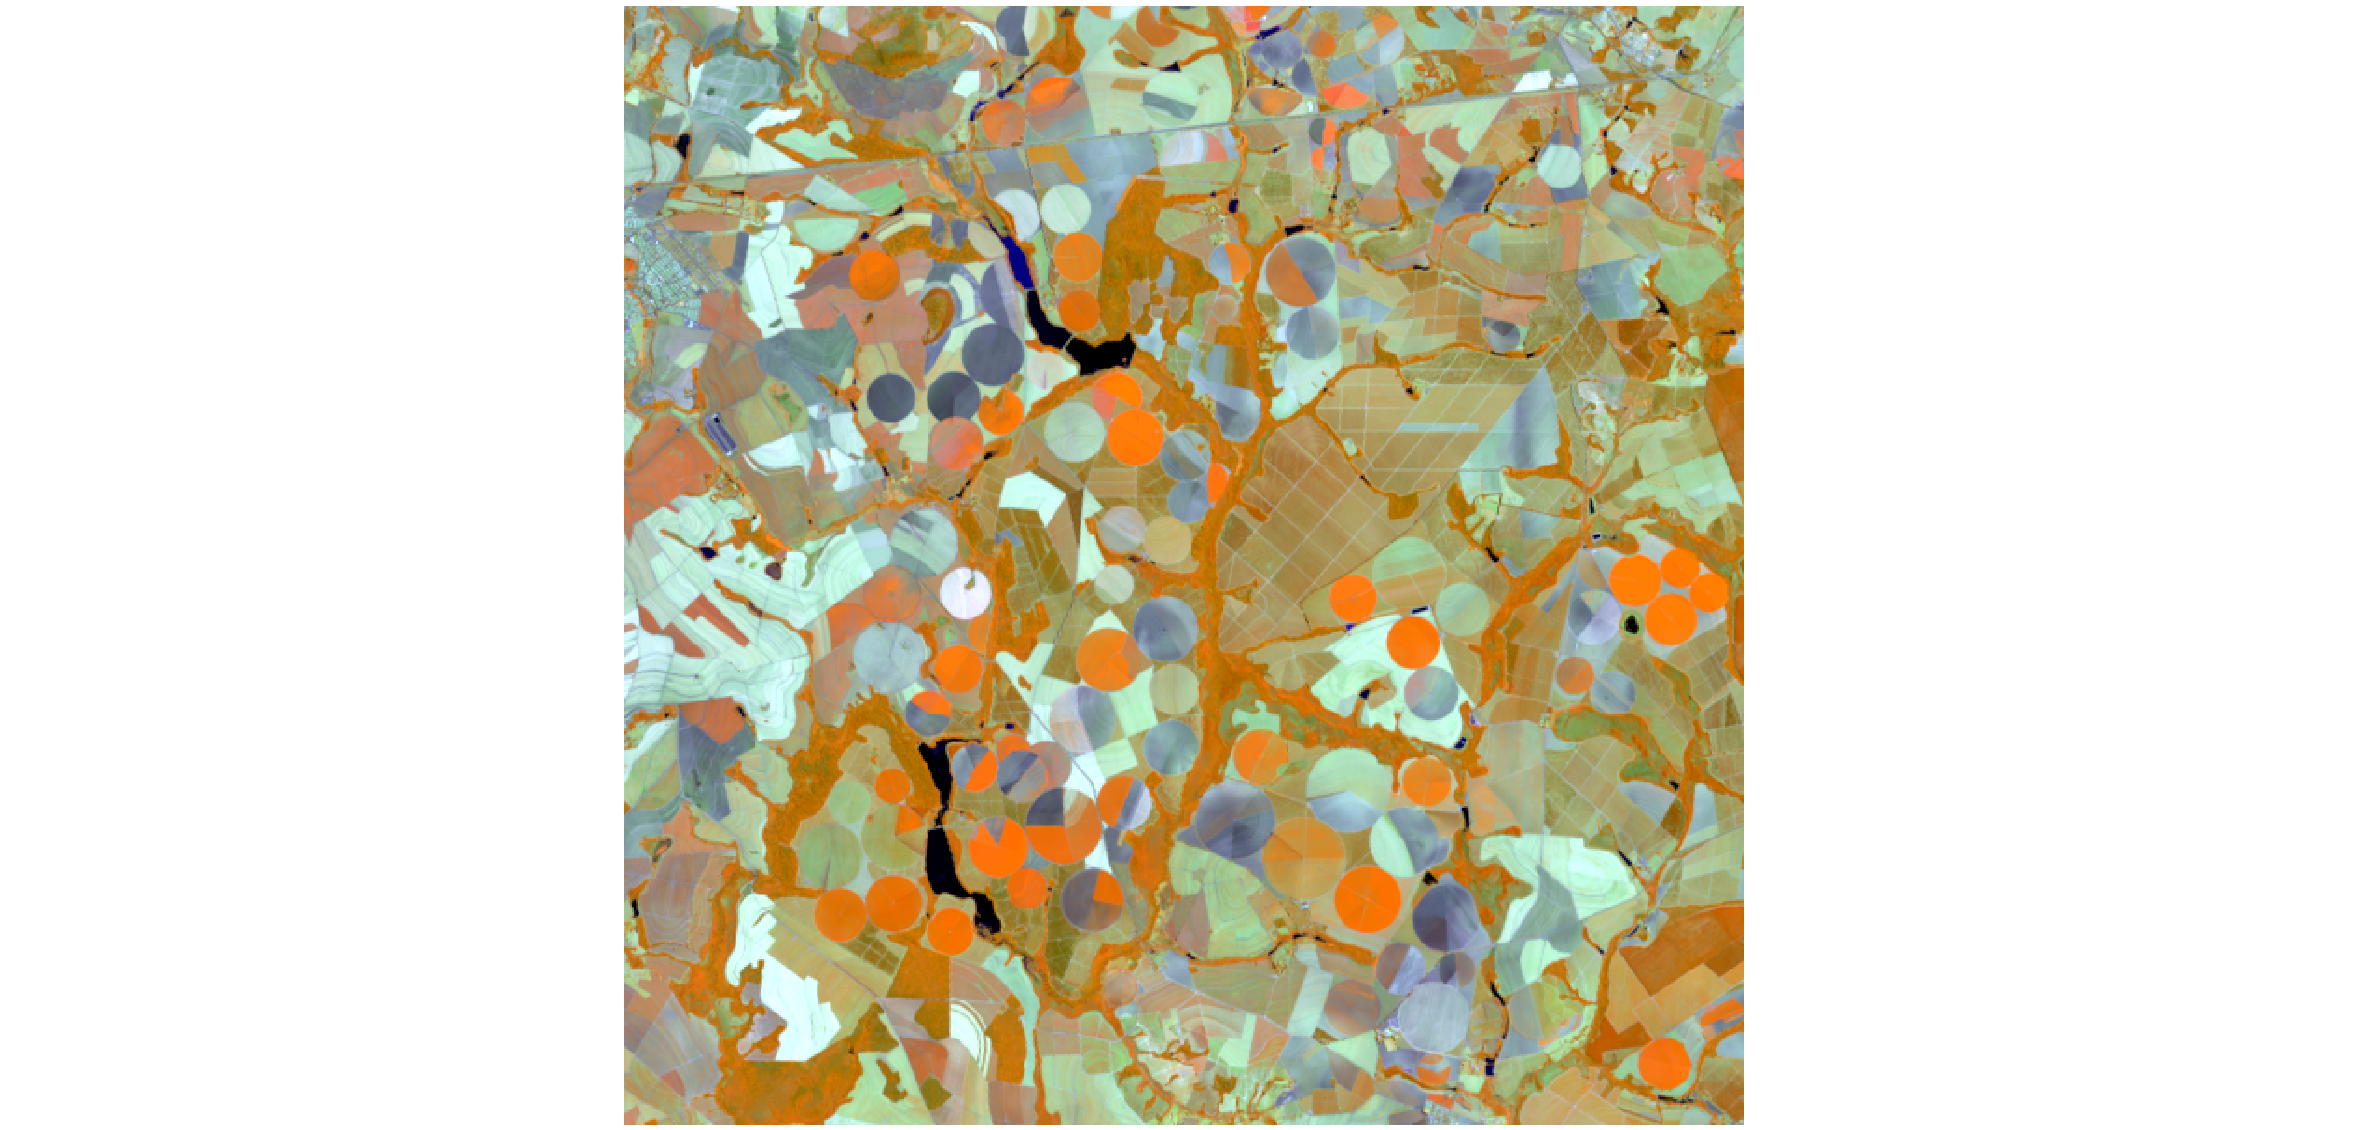
\includegraphics[width=1.\linewidth]{../images/rgb564}
		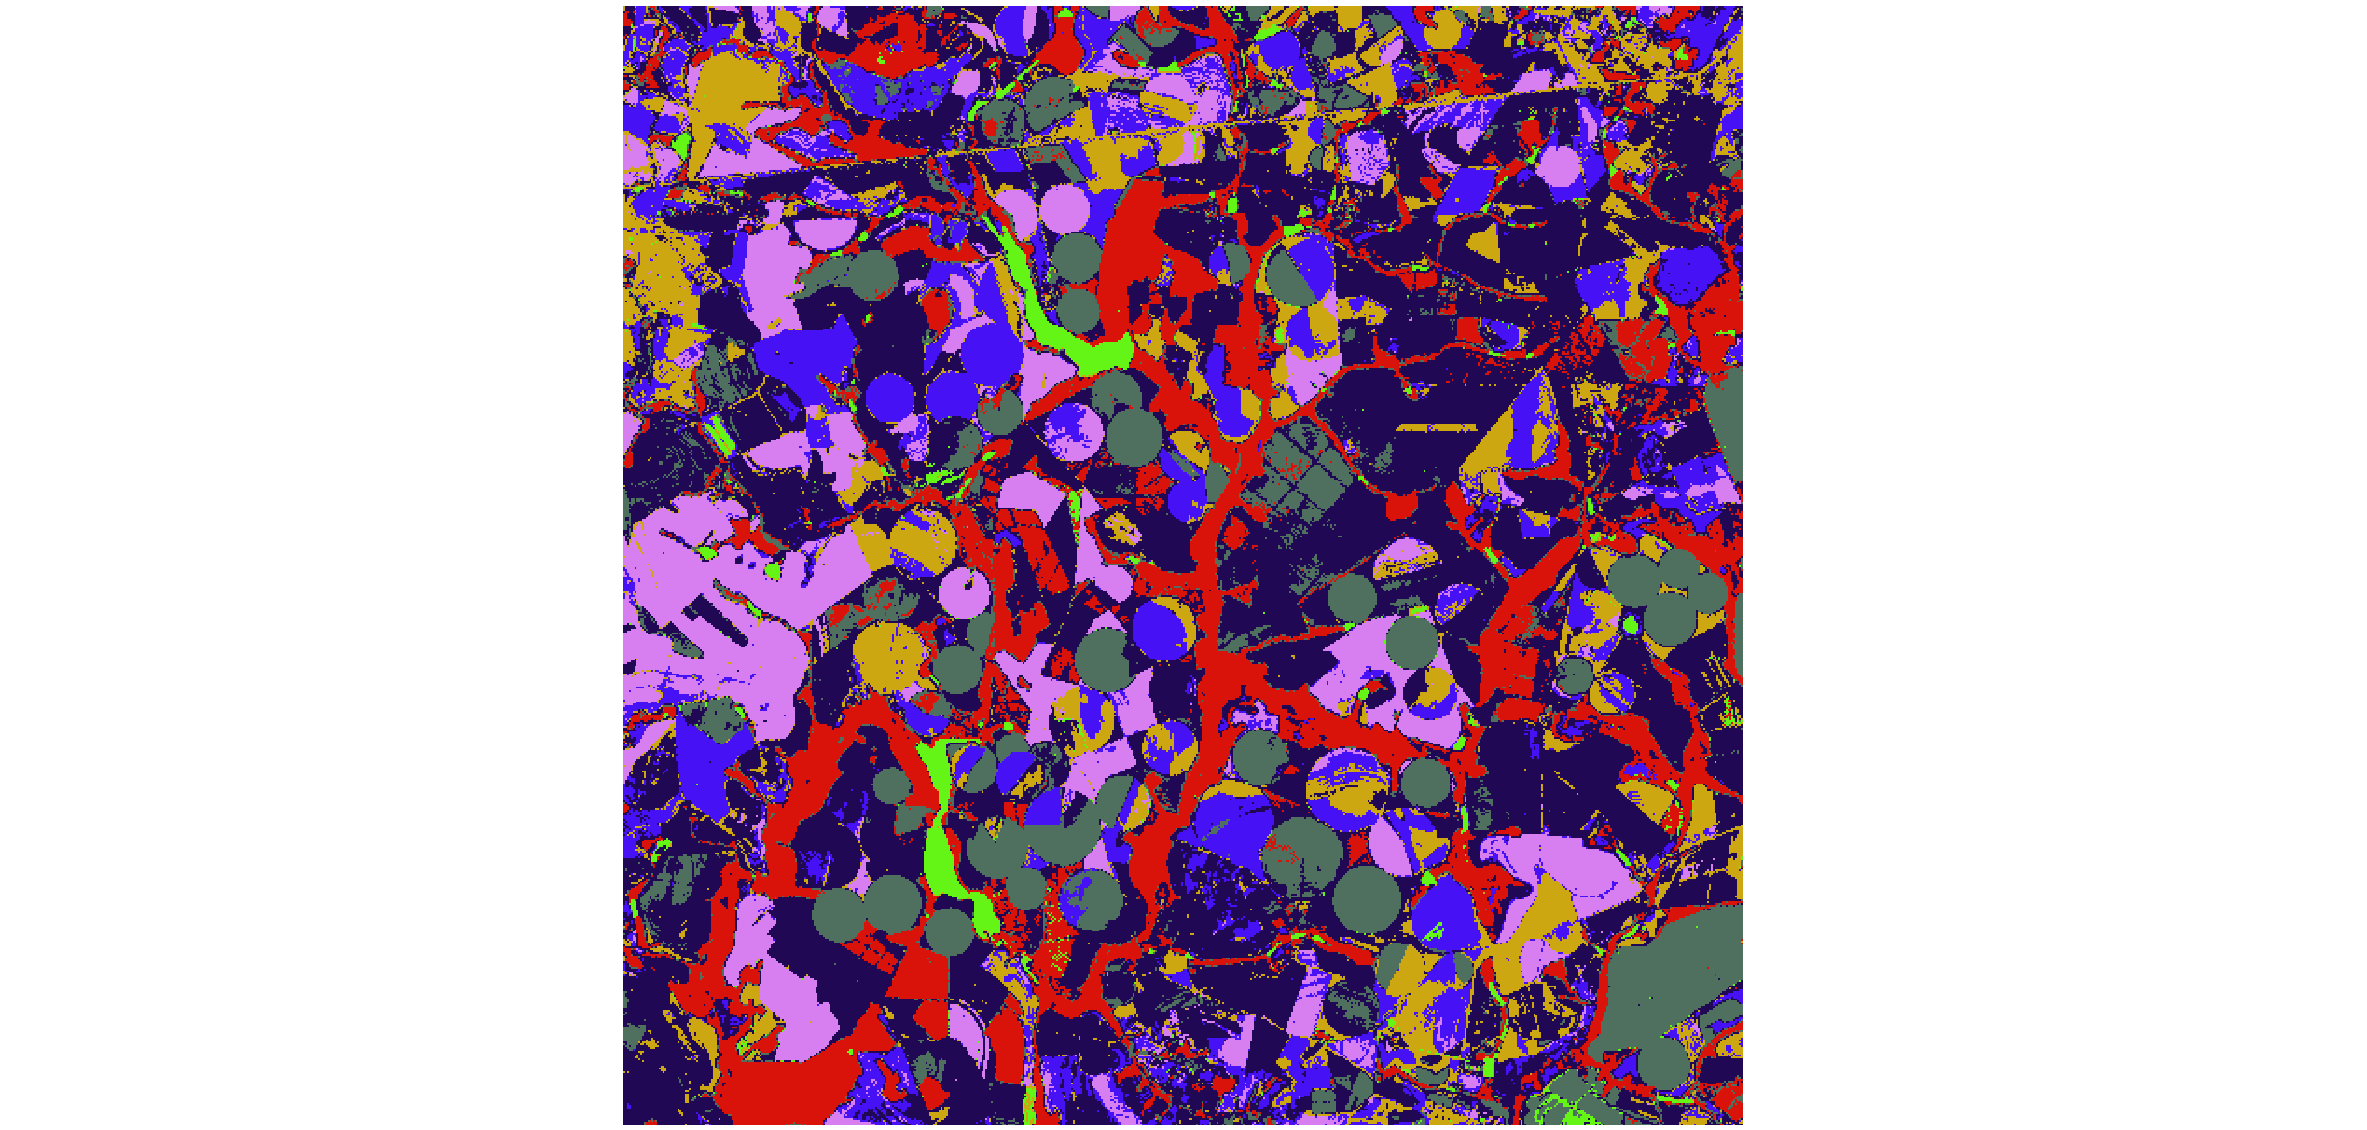
\includegraphics[width=1.\linewidth]{../images/classification}
		\caption{De cima para baixo temos uma composição cor verdadeira RGB432, seguida de uma composição falsa cor RGB564 e, por fim, uma captura da classificação supervisionada.}
	\end{figure}
	\section{Capturas de tela}
	\begin{figure}[H]
		\centering
		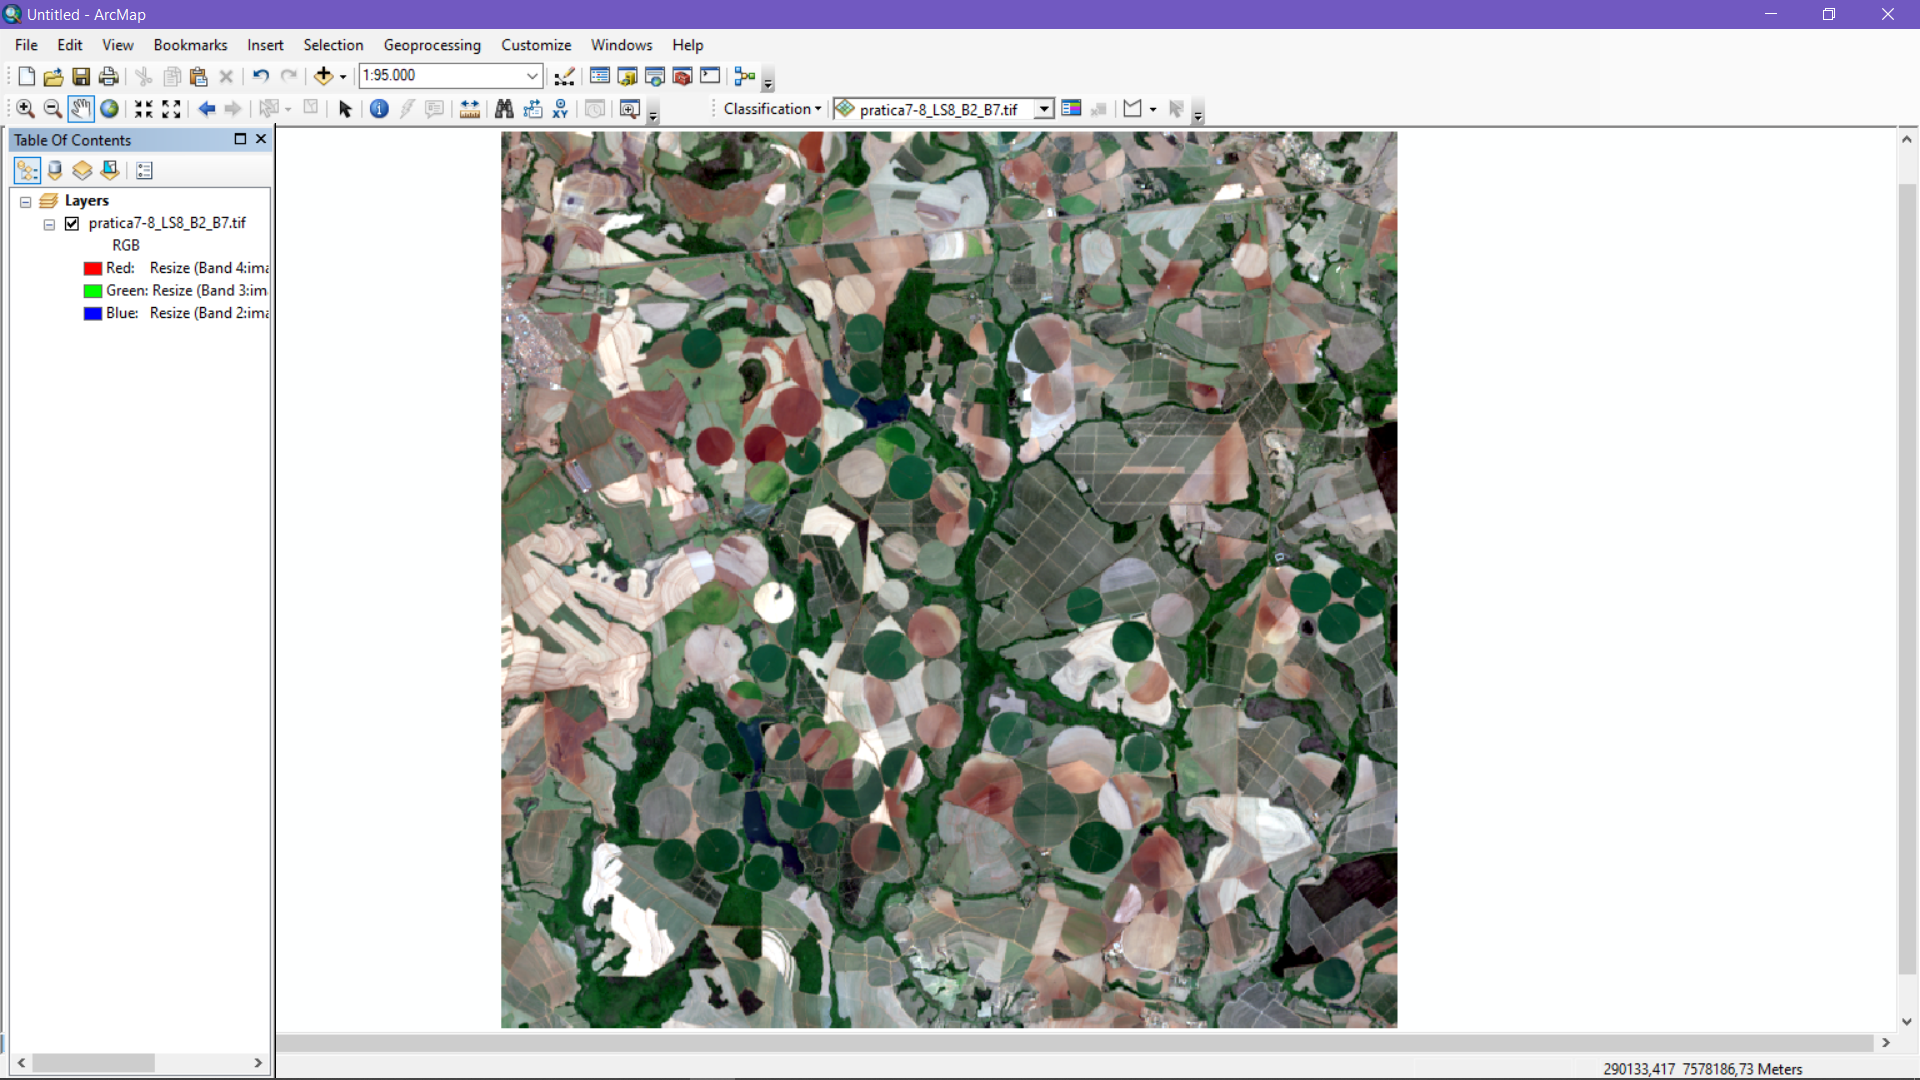
\includegraphics[width=1\linewidth]{../images/print_432}
		\caption{RGB432}
	\end{figure}
	\begin{figure}[H]
		\centering
		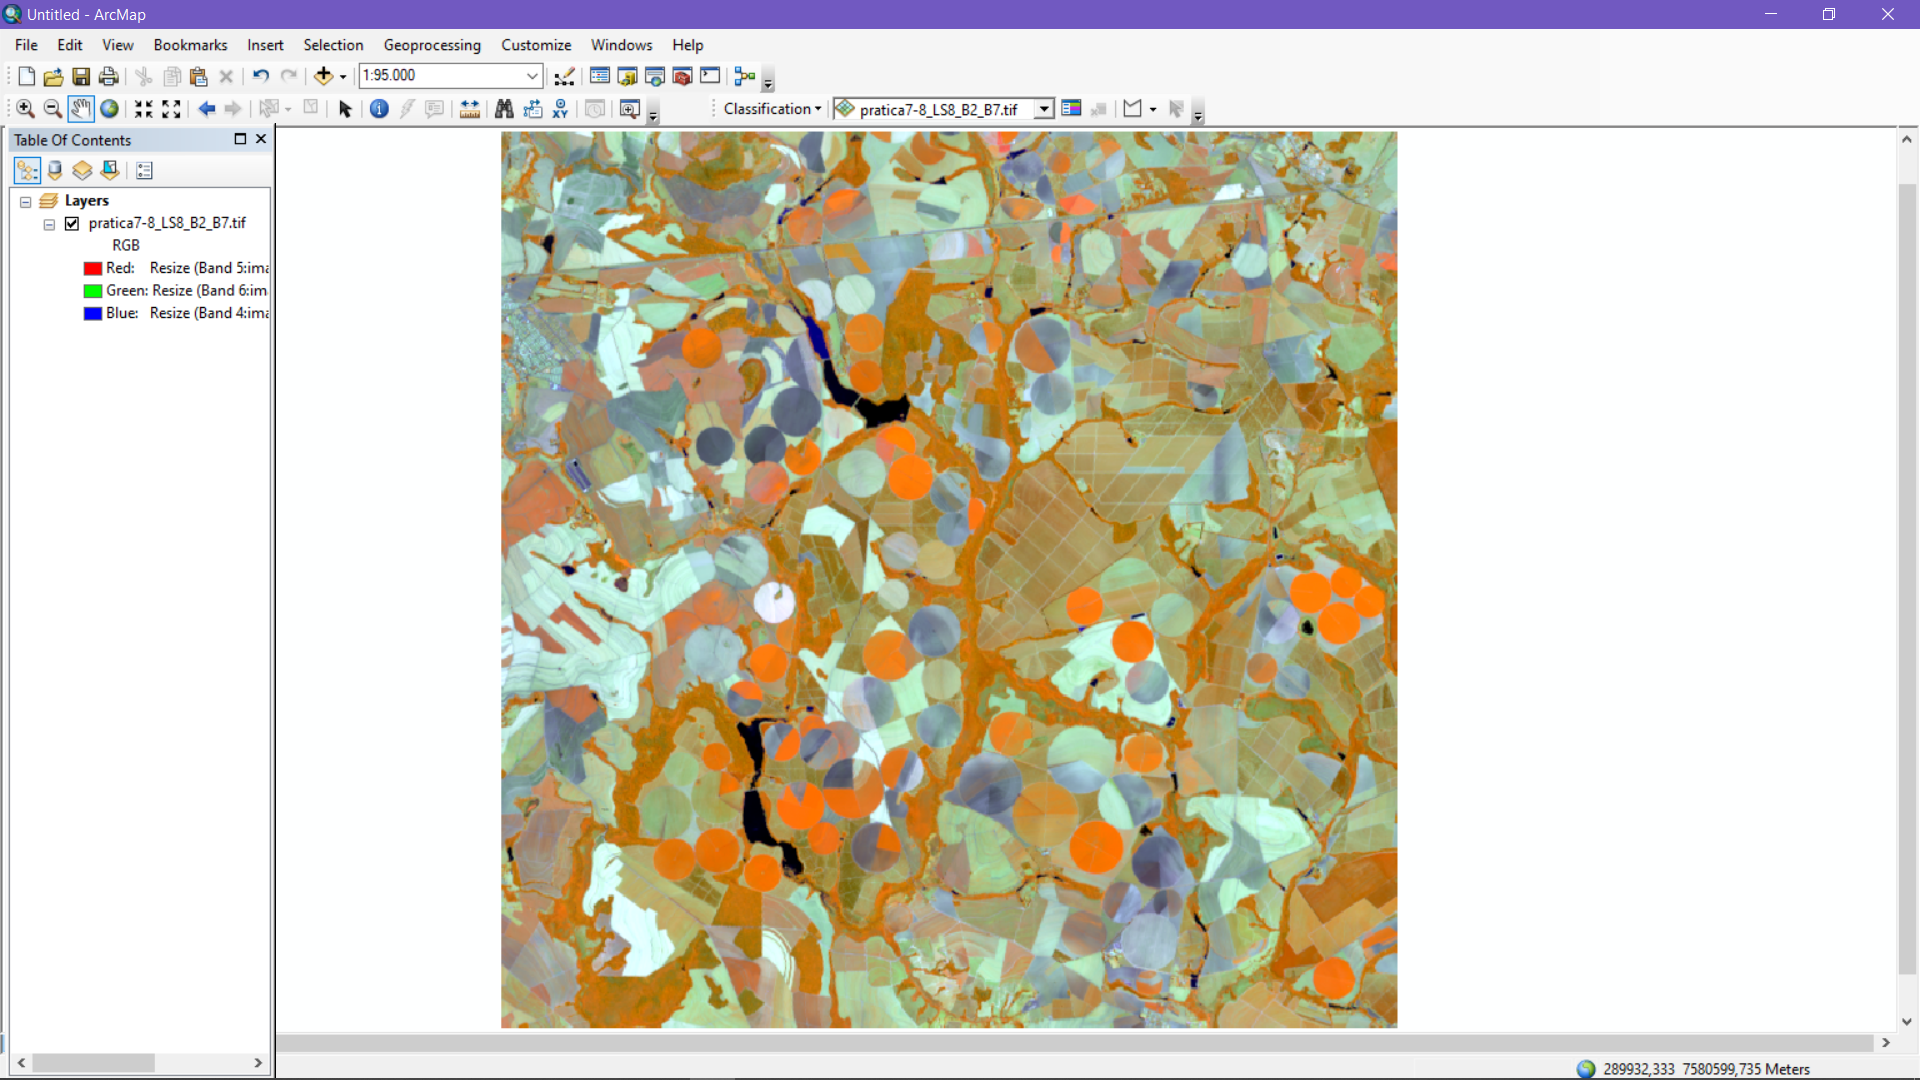
\includegraphics[width=1\linewidth]{../images/print_564}
		\caption{RGB564}
	\end{figure}
	\begin{figure}[H]
		\centering
		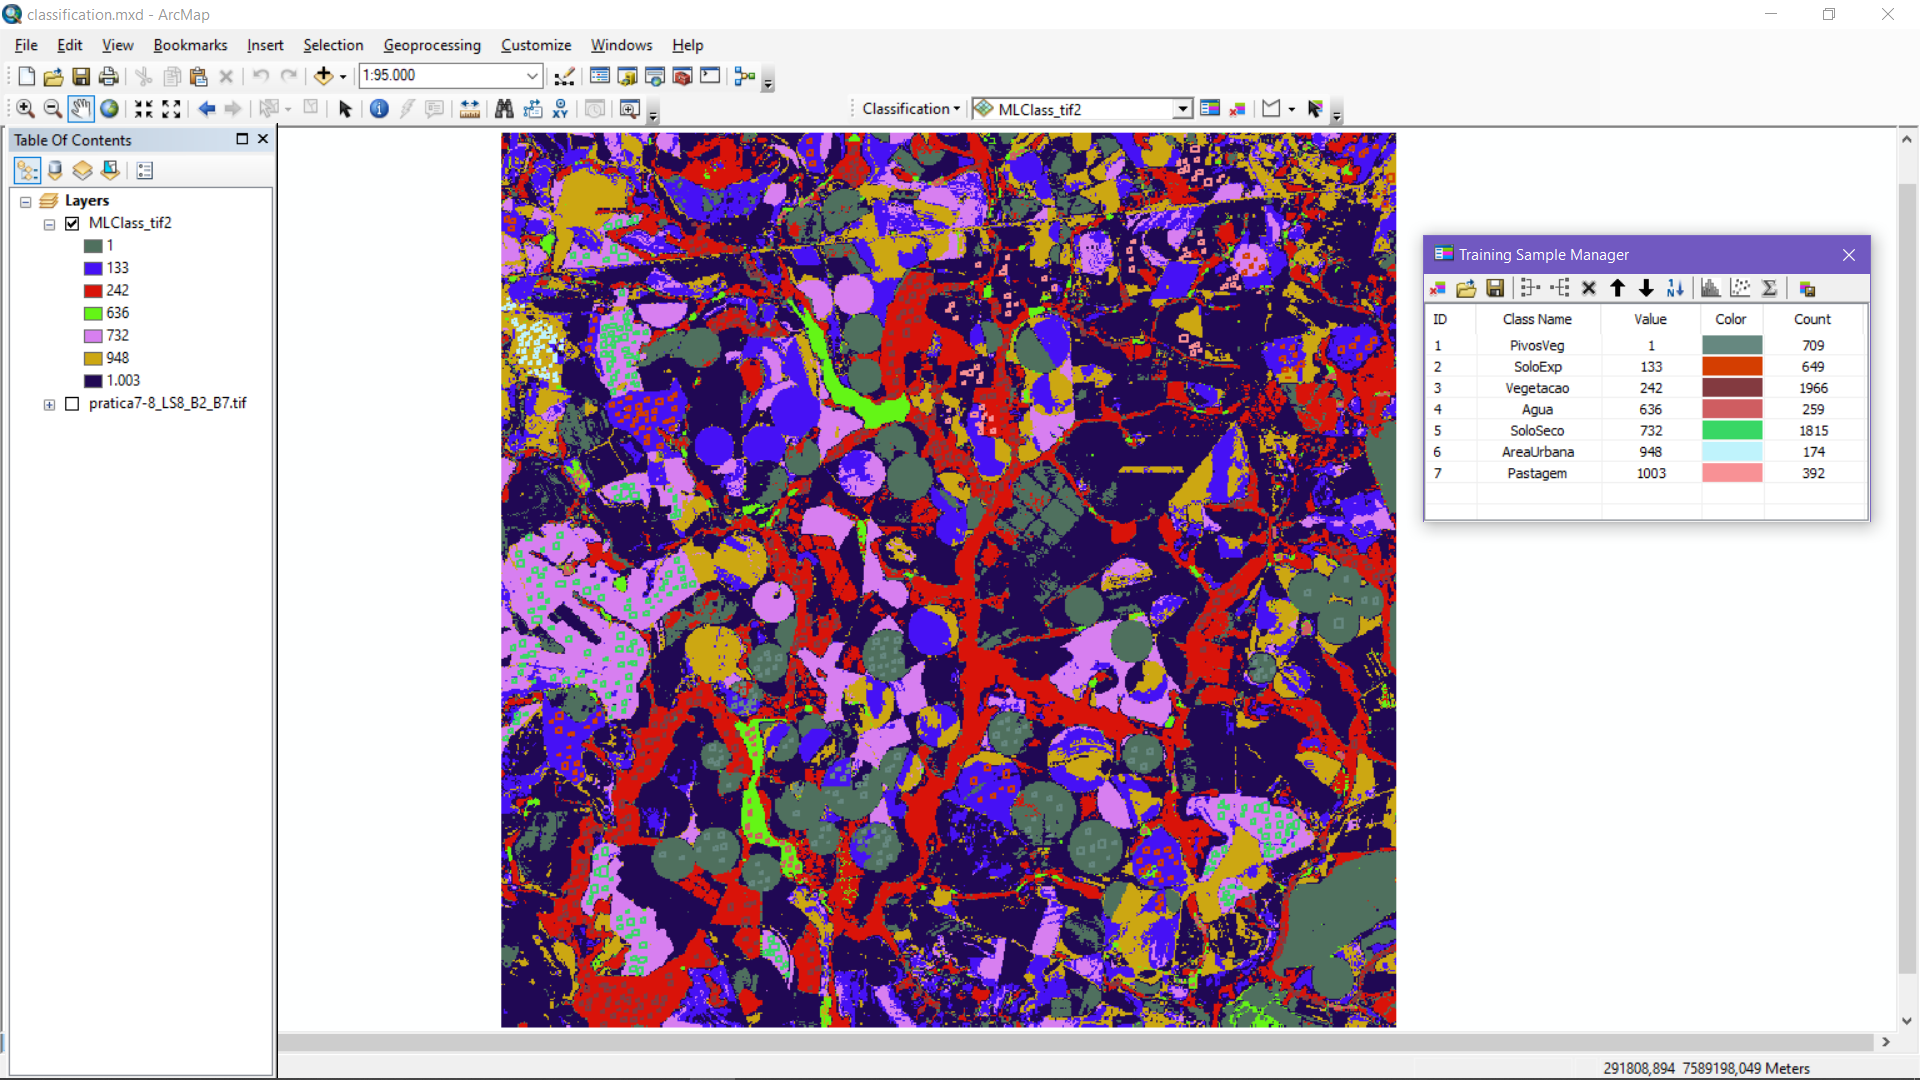
\includegraphics[width=1\linewidth]{../images/print_classification}
		\caption{Classificação supervisionada}
	\end{figure}
	\newpage
	\section{Alvos sob diferentes perspectivas de tratamento}
	\textbf{Obs:} Da esquerda para a direita temos uma composição cor verdadeira no RGB432, cor falsa no RGB564 e uma classificação supervisionada de máxima verossimilhança.
	
	\begin{figure}[H]
		\centering
		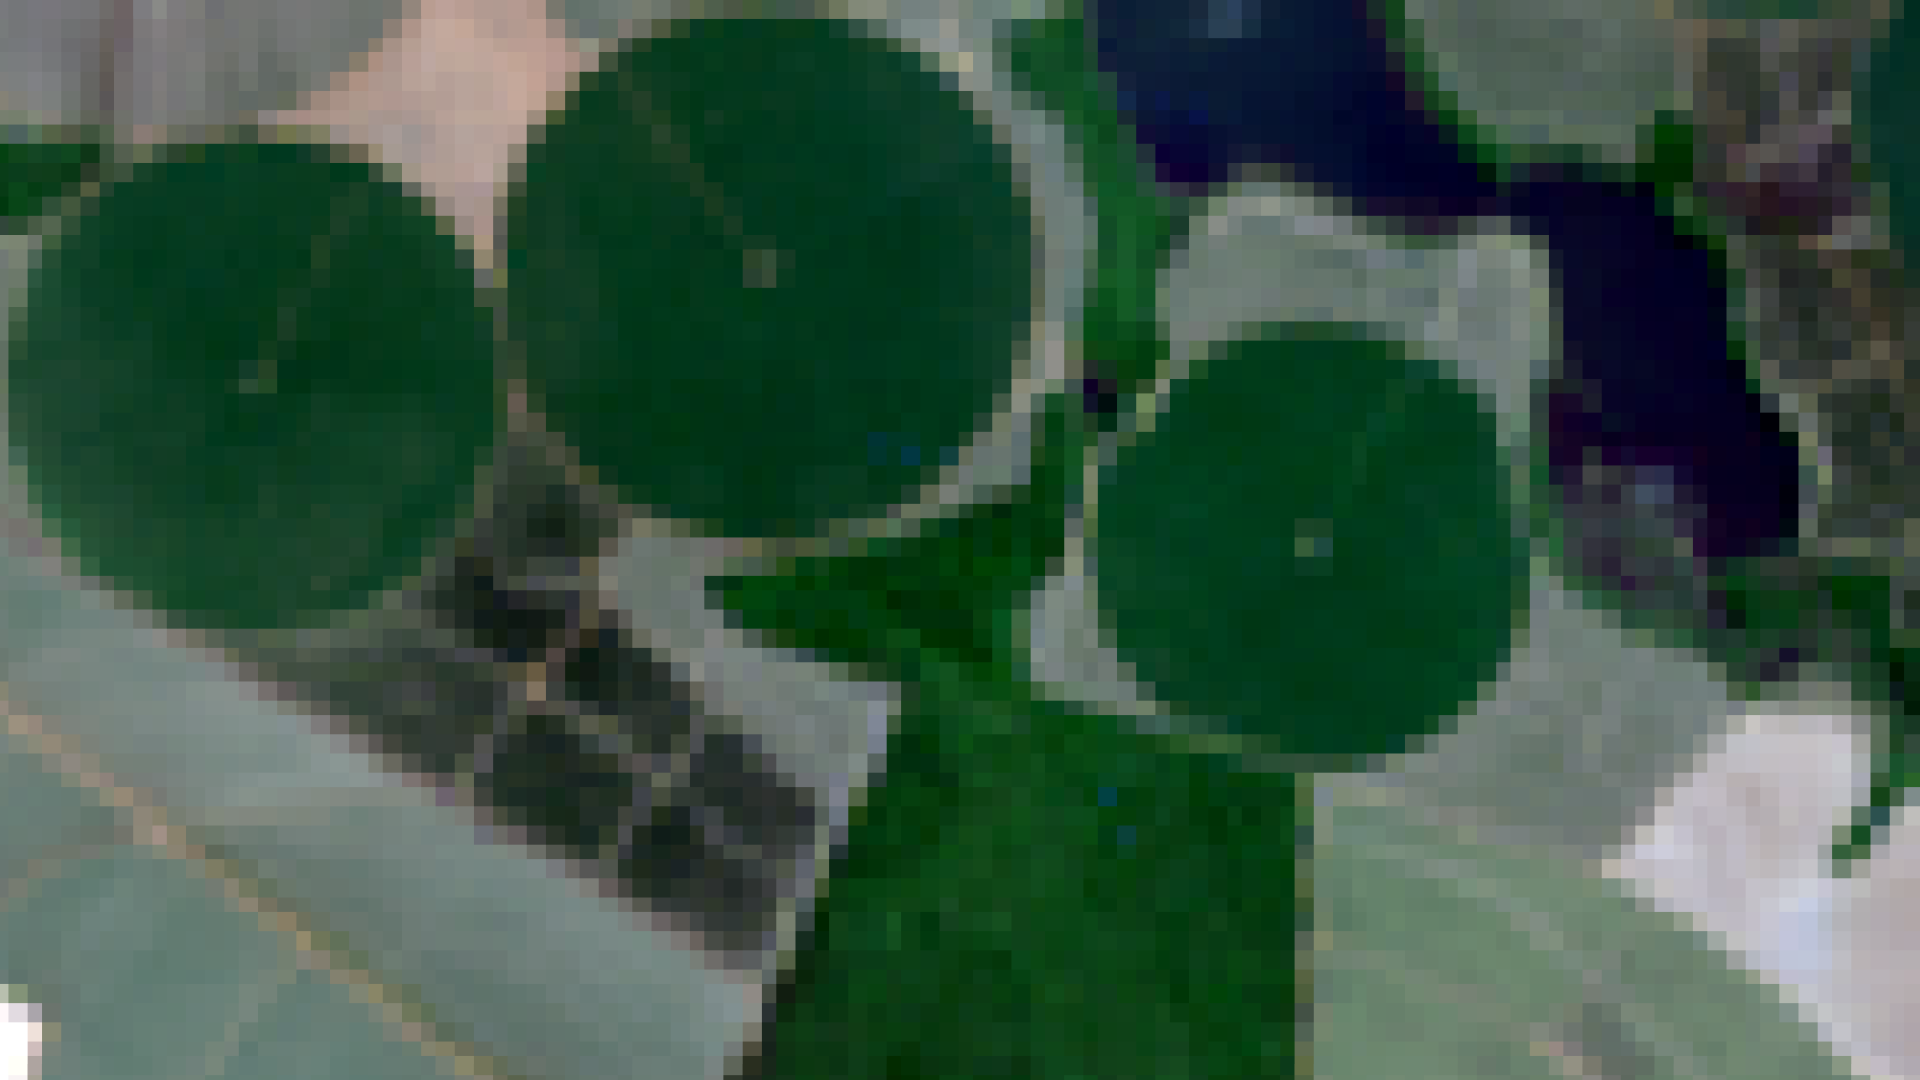
\includegraphics[width=.32\linewidth]{../images/pivosVeg/432}
		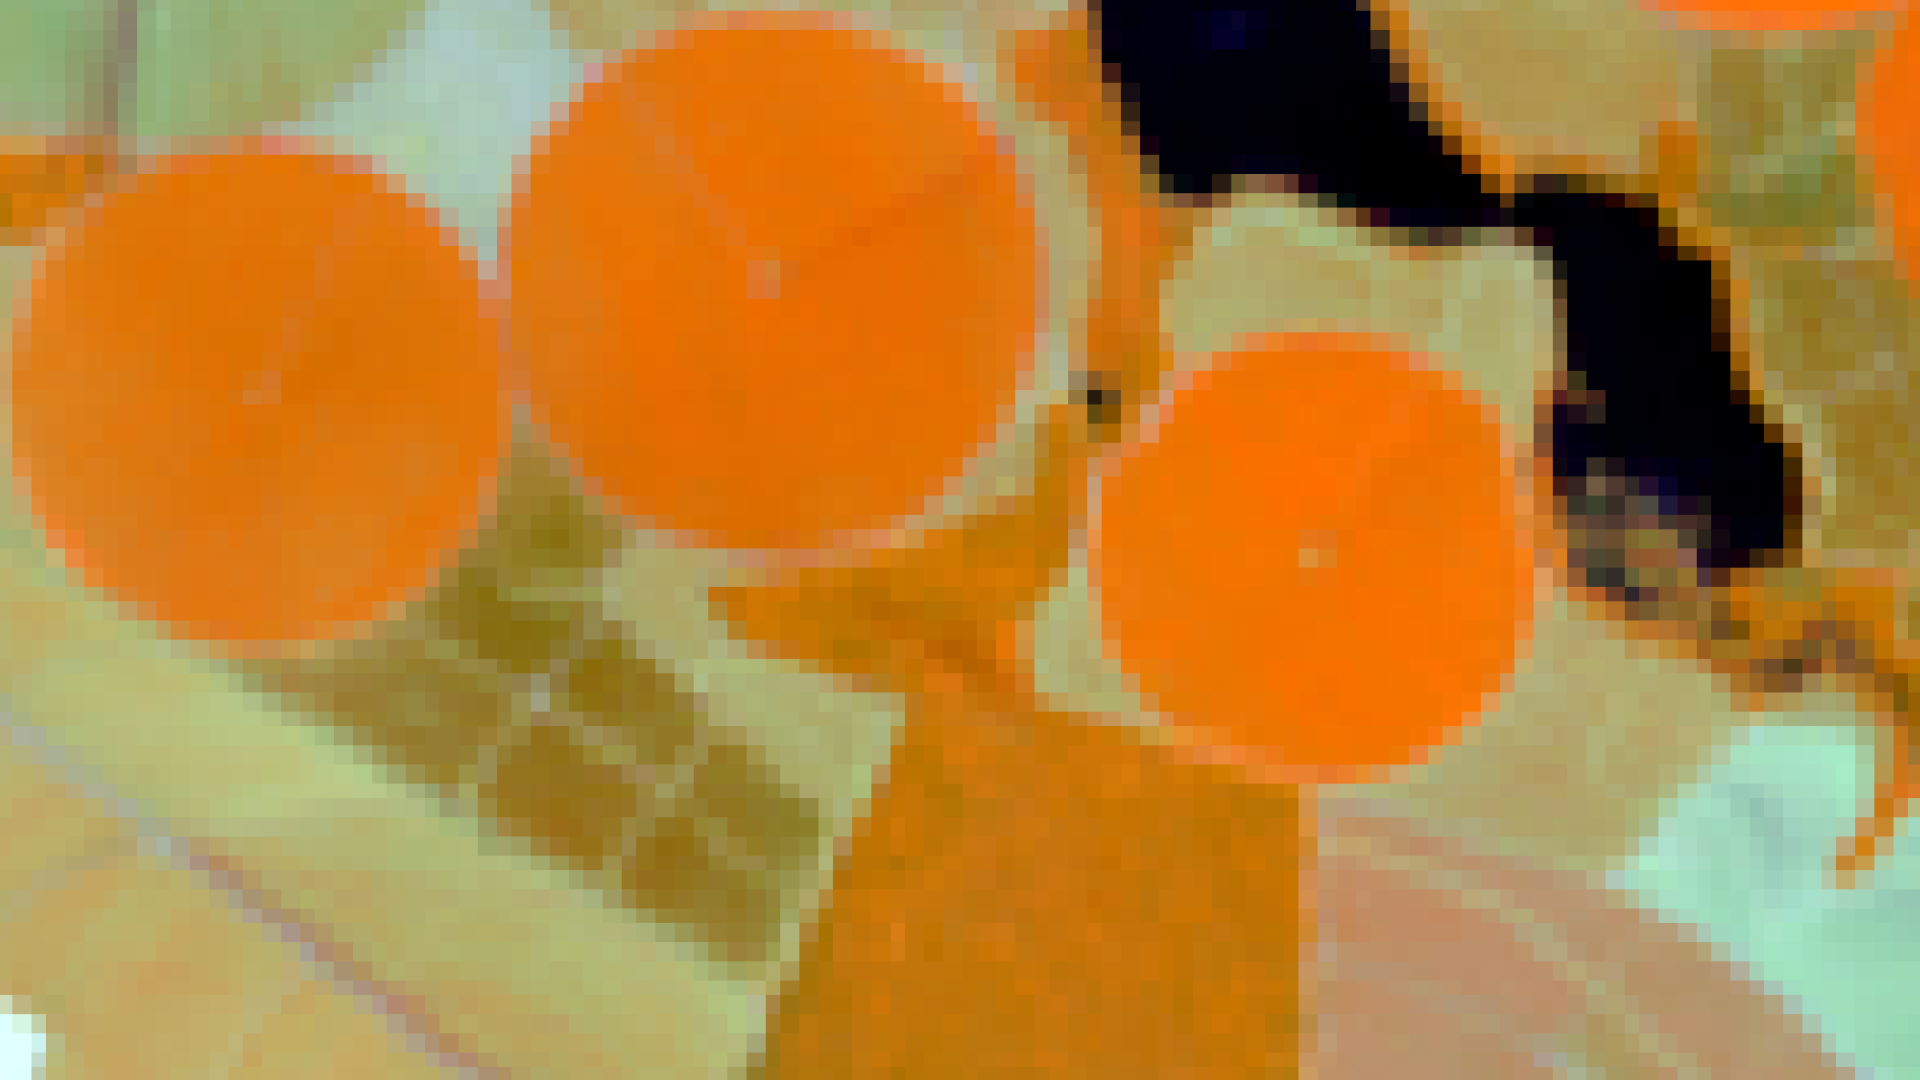
\includegraphics[width=.32\linewidth]{../images/pivosVeg/564}
		
\includegraphics[width=.32\linewidth]{../images/pivosVeg/class}
		\caption{Pivôs centrais}
	\end{figure}
	\begin{figure}[H]
		\centering
		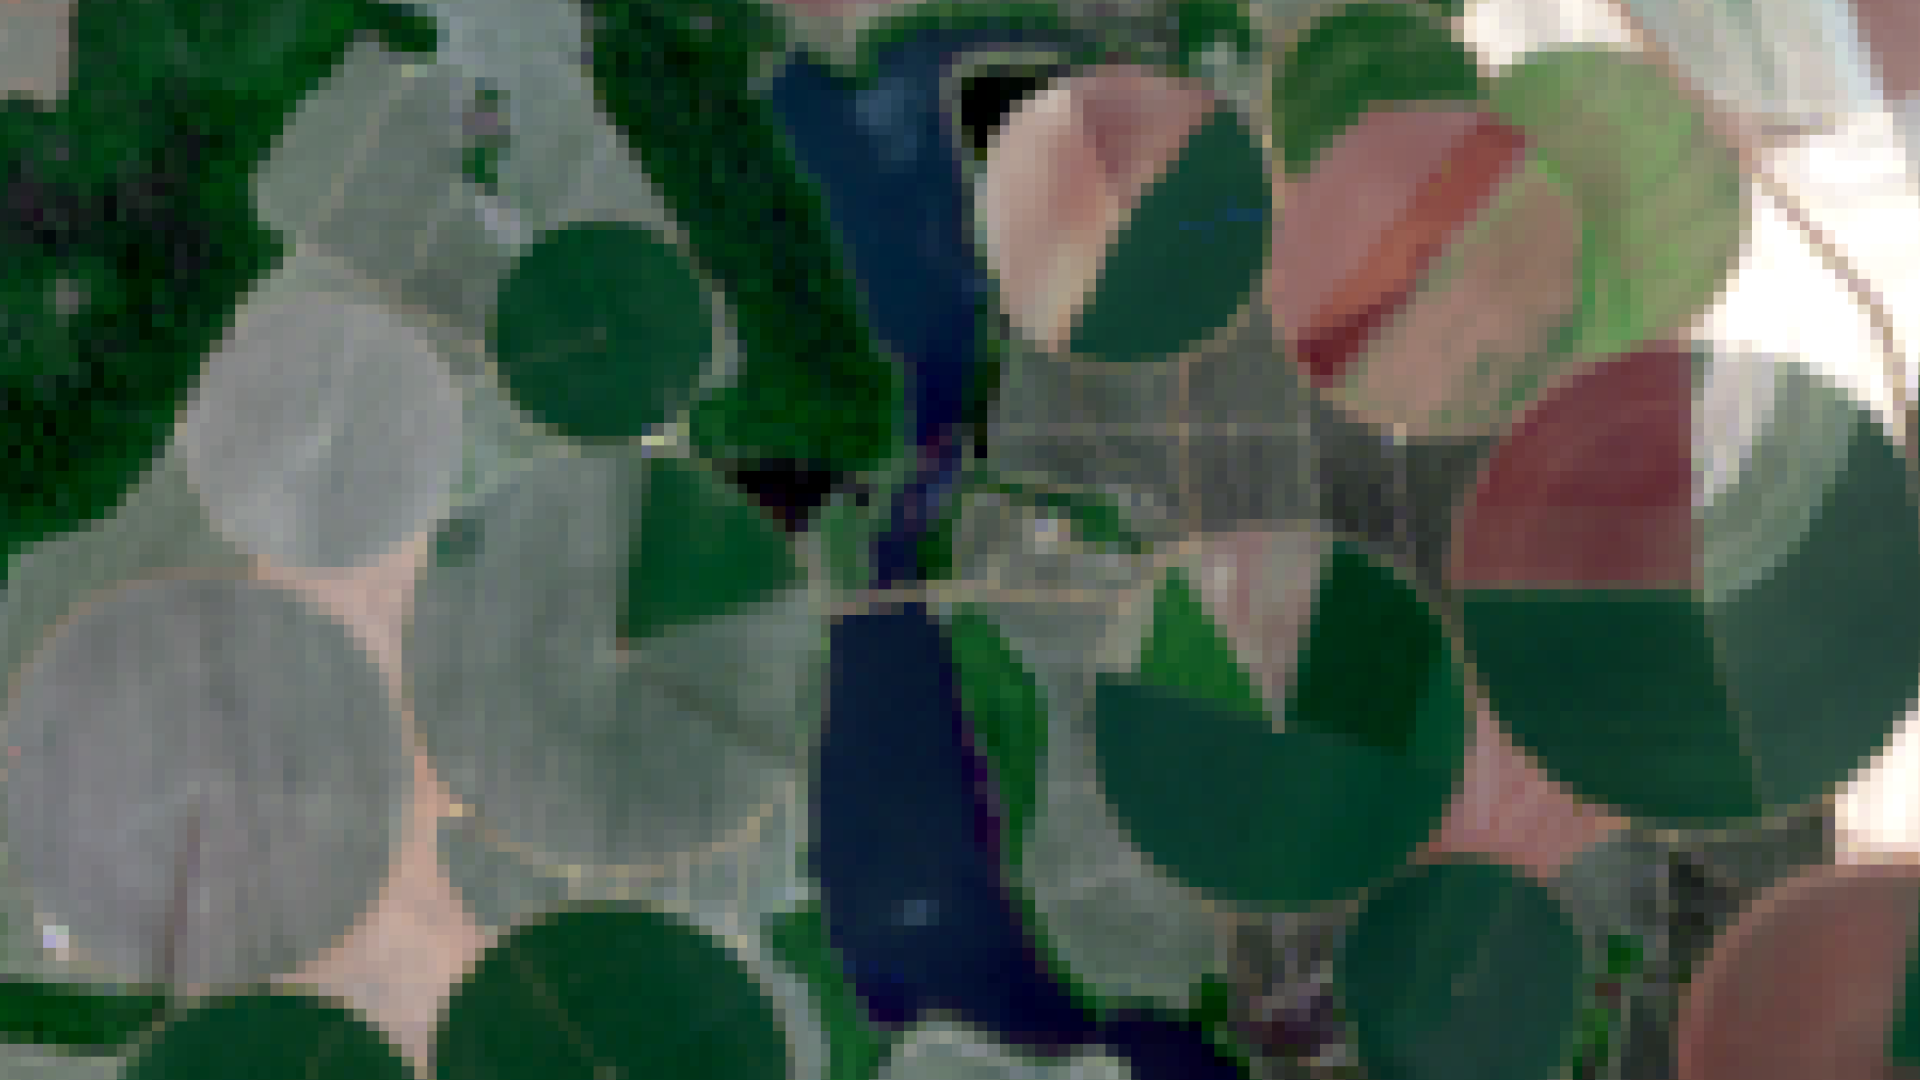
\includegraphics[width=.32\linewidth]{../images/agua/432}
		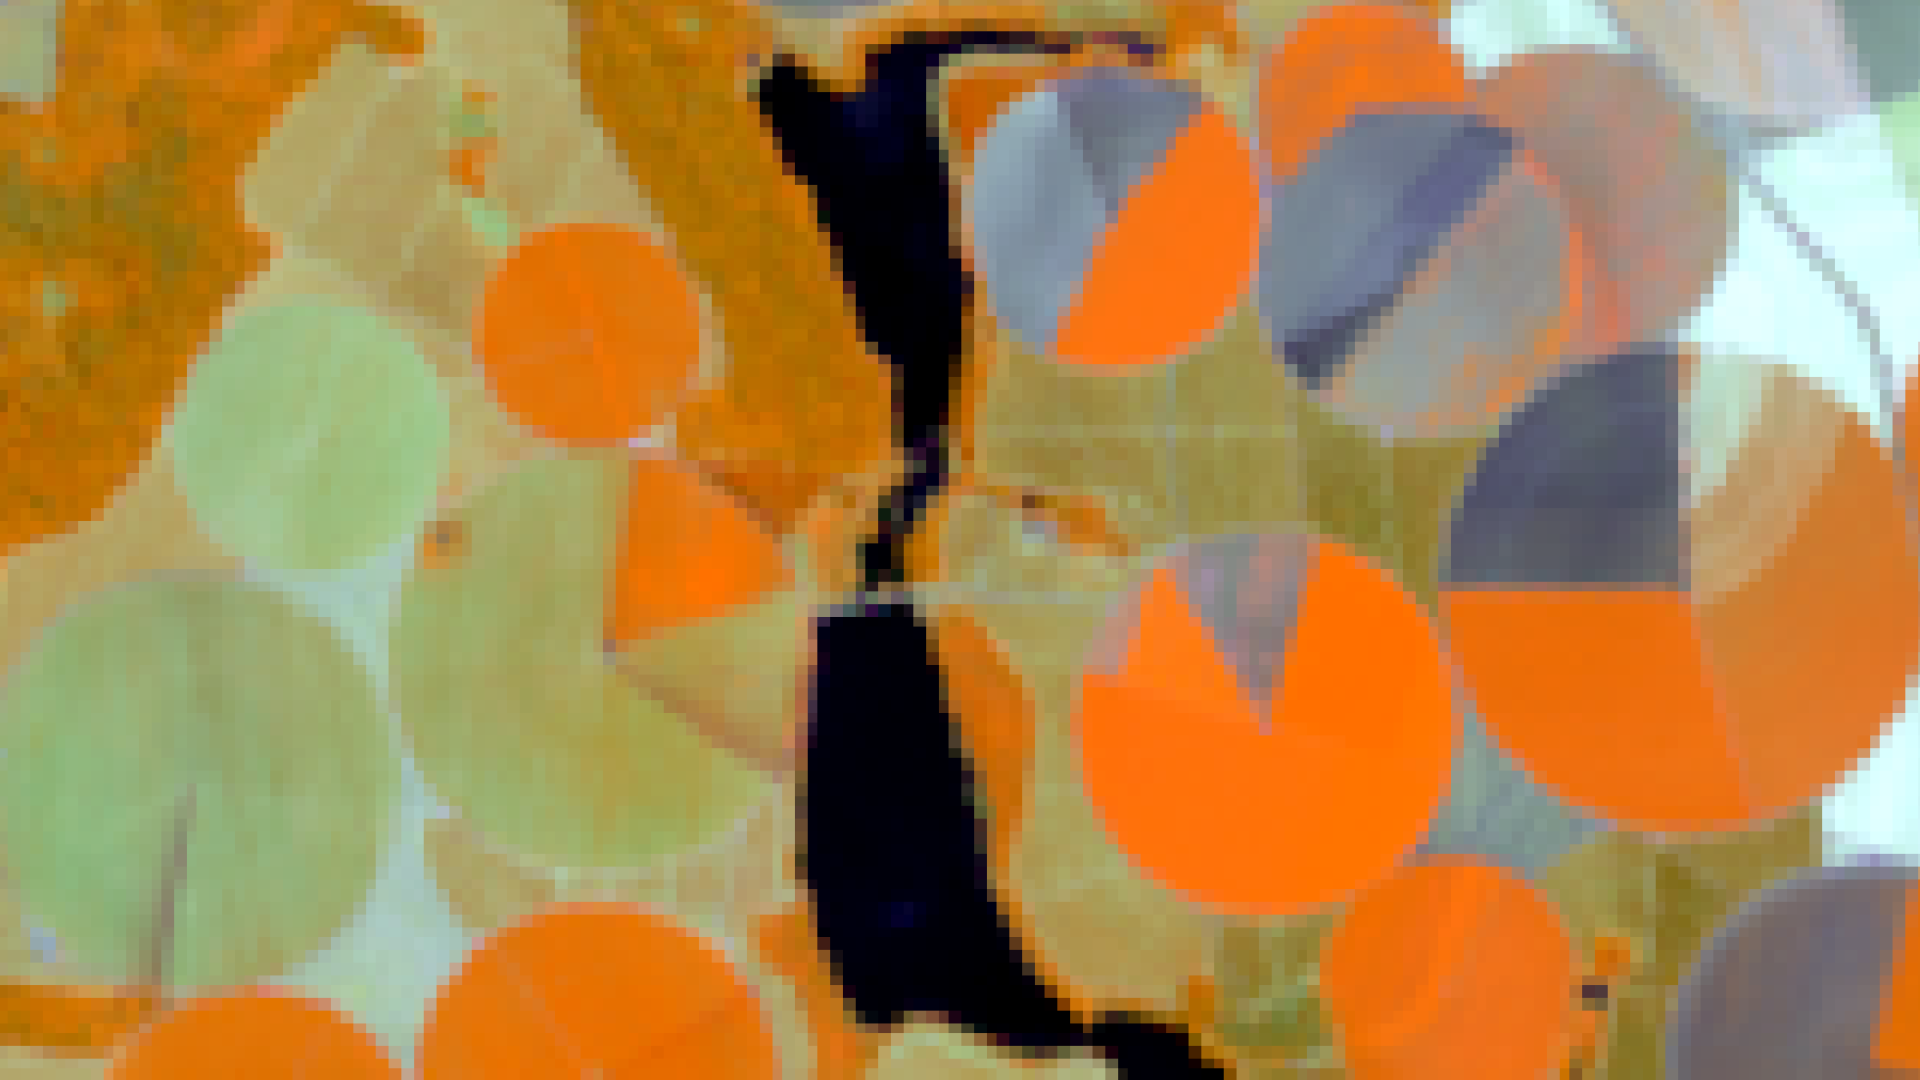
\includegraphics[width=.32\linewidth]{../images/agua/564}
		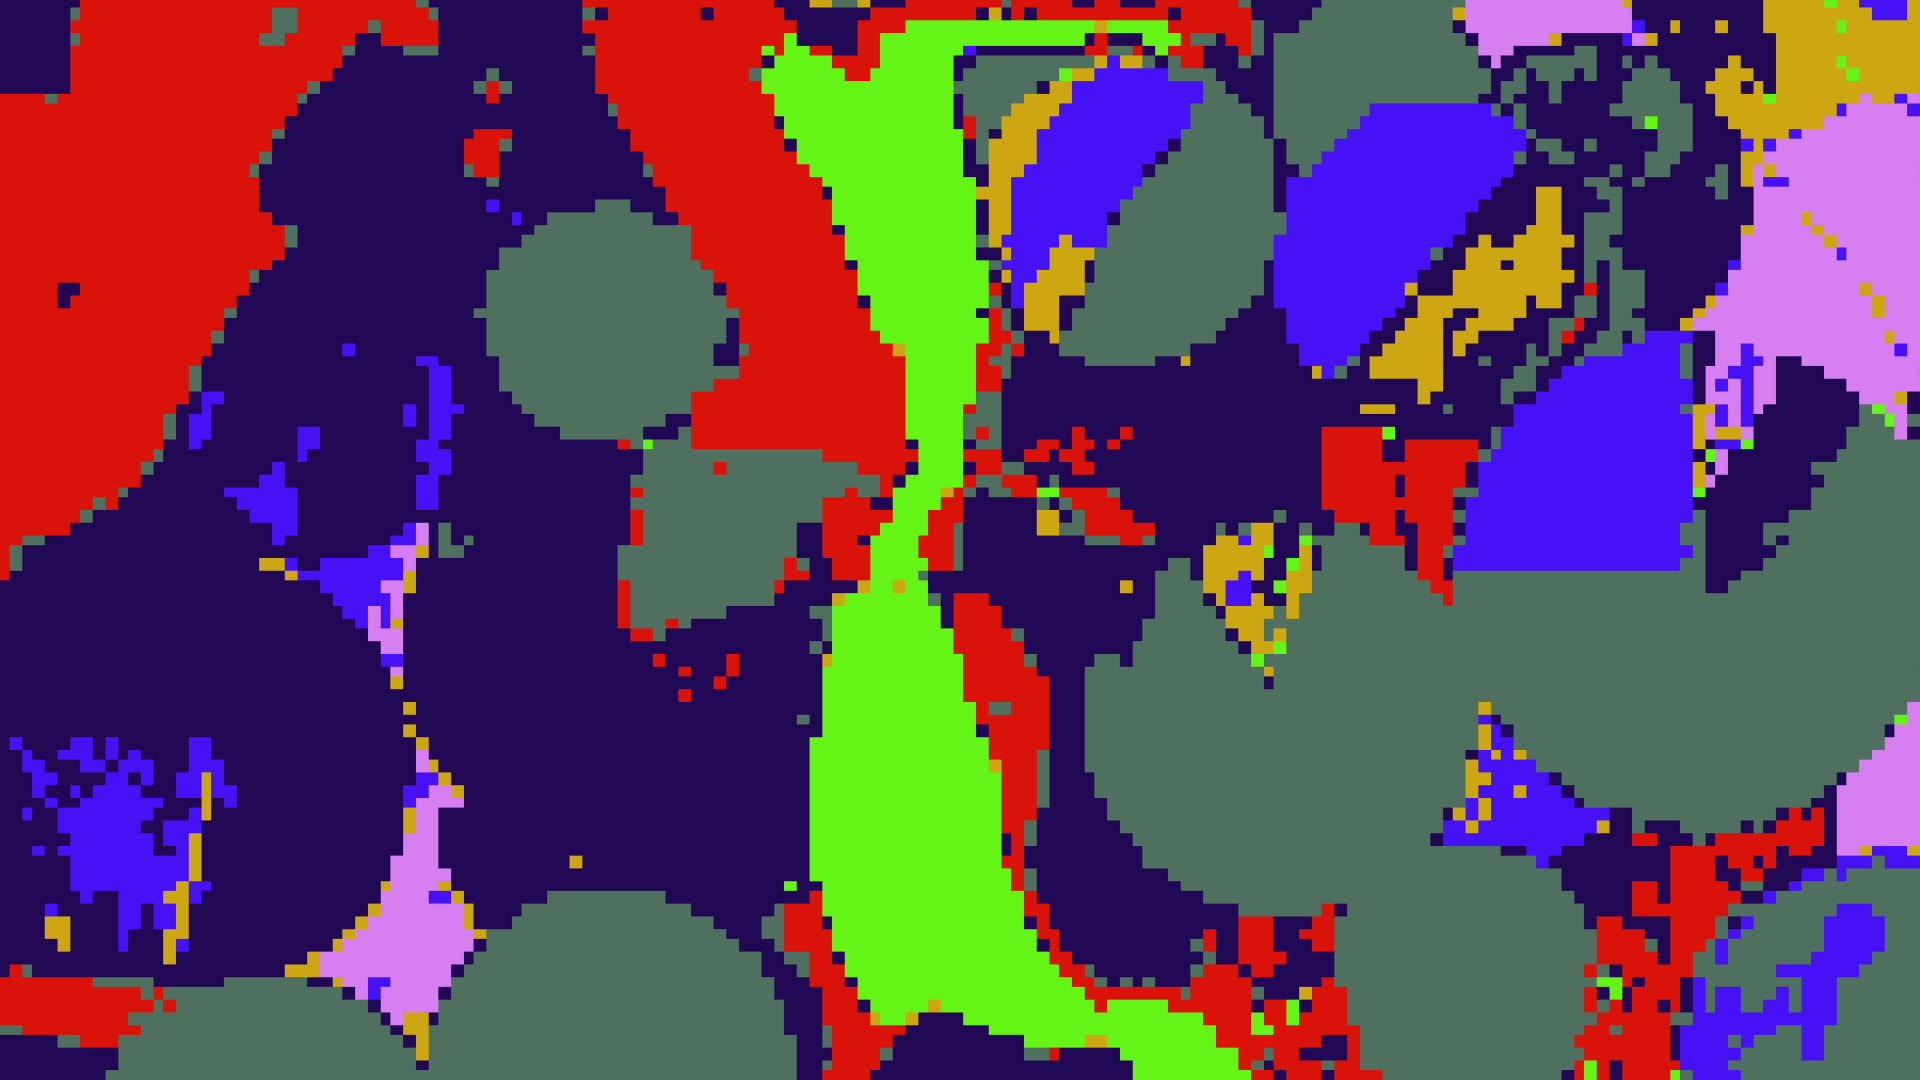
\includegraphics[width=.32\linewidth]{../images/agua/class}
		\caption{Corpos d'água}
	\end{figure}
	\begin{figure}[H]
		\centering
		\includegraphics[width=.32\linewidth]{../images/soloSecoExp/432}
		\includegraphics[width=.32\linewidth]{../images/soloSecoExp/564}
		\includegraphics[width=.32\linewidth]{../images/soloSecoExp/class}
		\caption{Solo exposto com menor umidade}
	\end{figure}
	\begin{figure}[H]
		\centering
		\includegraphics[width=.32\linewidth]{../images/soloUmidoExp/432}
		\includegraphics[width=.32\linewidth]{../images/soloUmidoExp/564}
		\includegraphics[width=.32\linewidth]{../images/soloUmidoExp/class}
		\caption{Solo exposto com maior umidade}
	\end{figure}
	\begin{figure}[H]
		\centering
		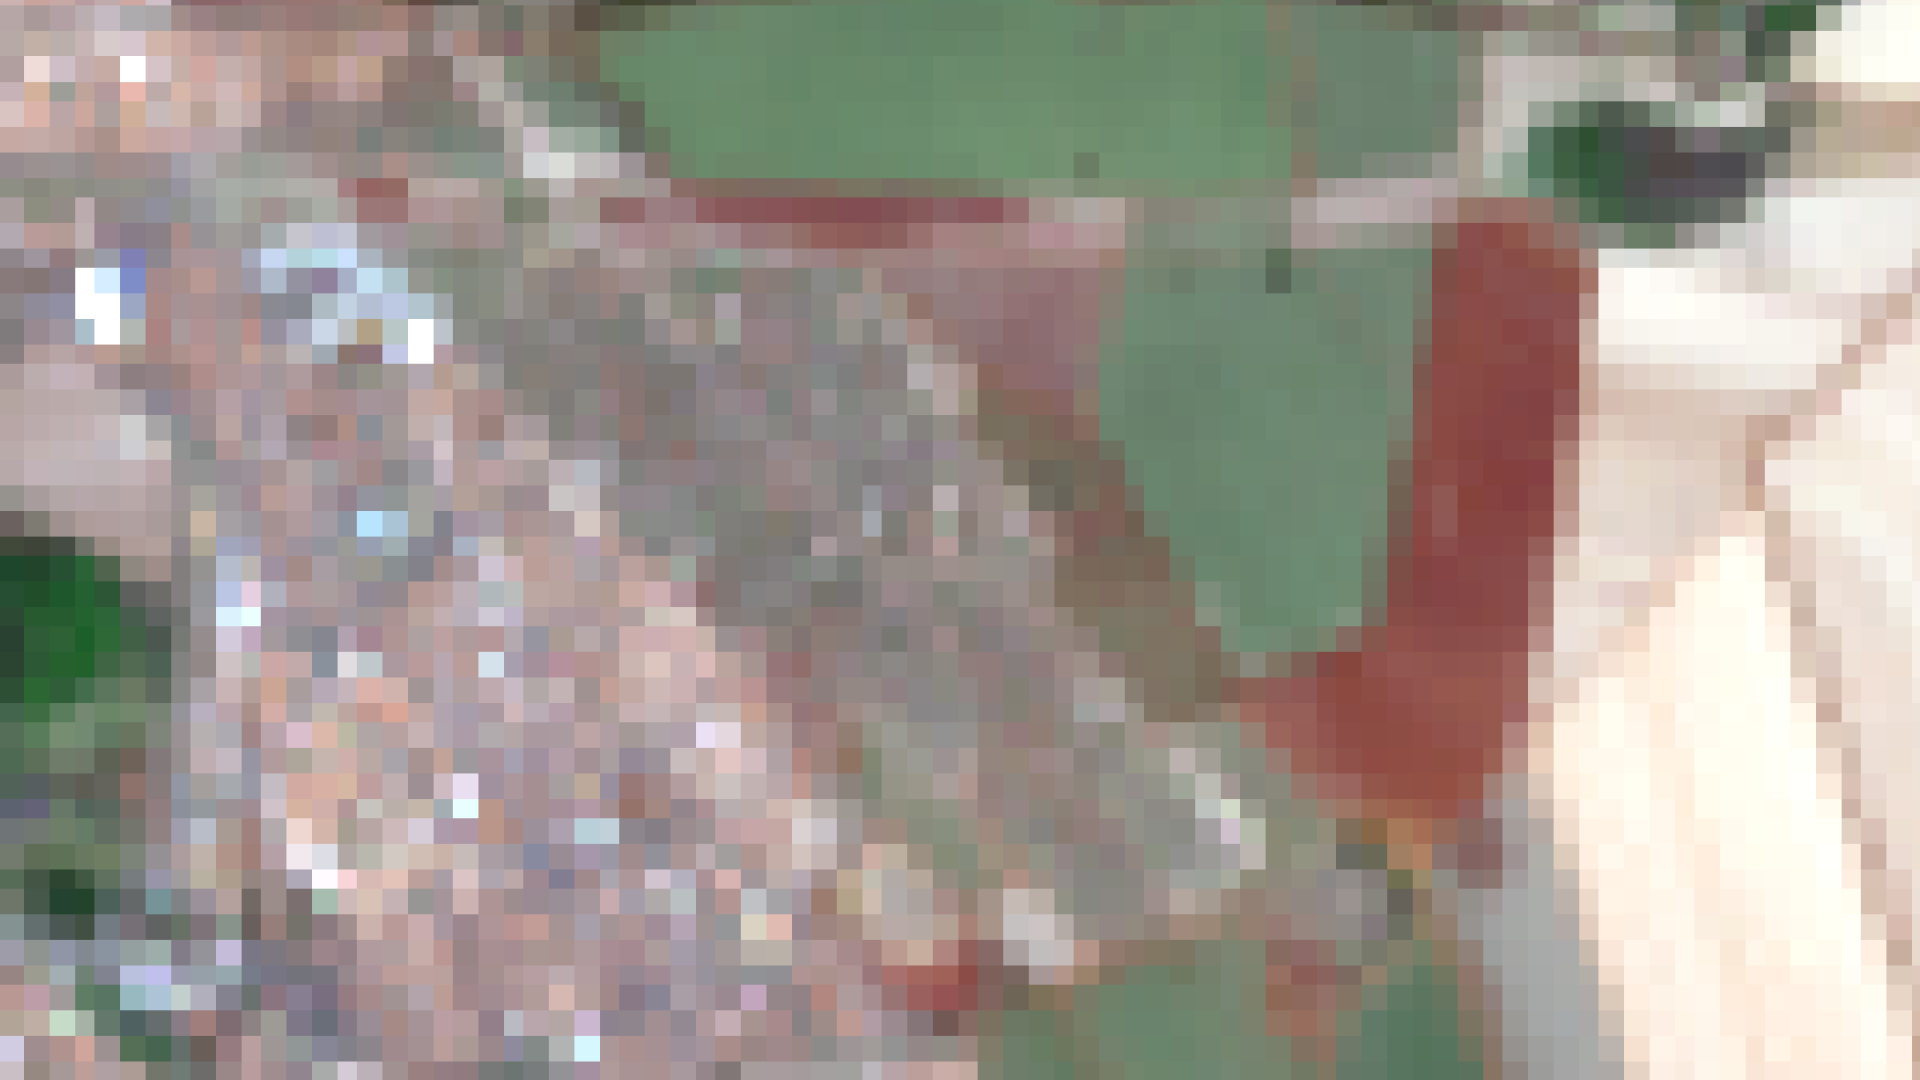
\includegraphics[width=.32\linewidth]{../images/areaUrbana/432}
		\includegraphics[width=.32\linewidth]{../images/areaUrbana/564}
		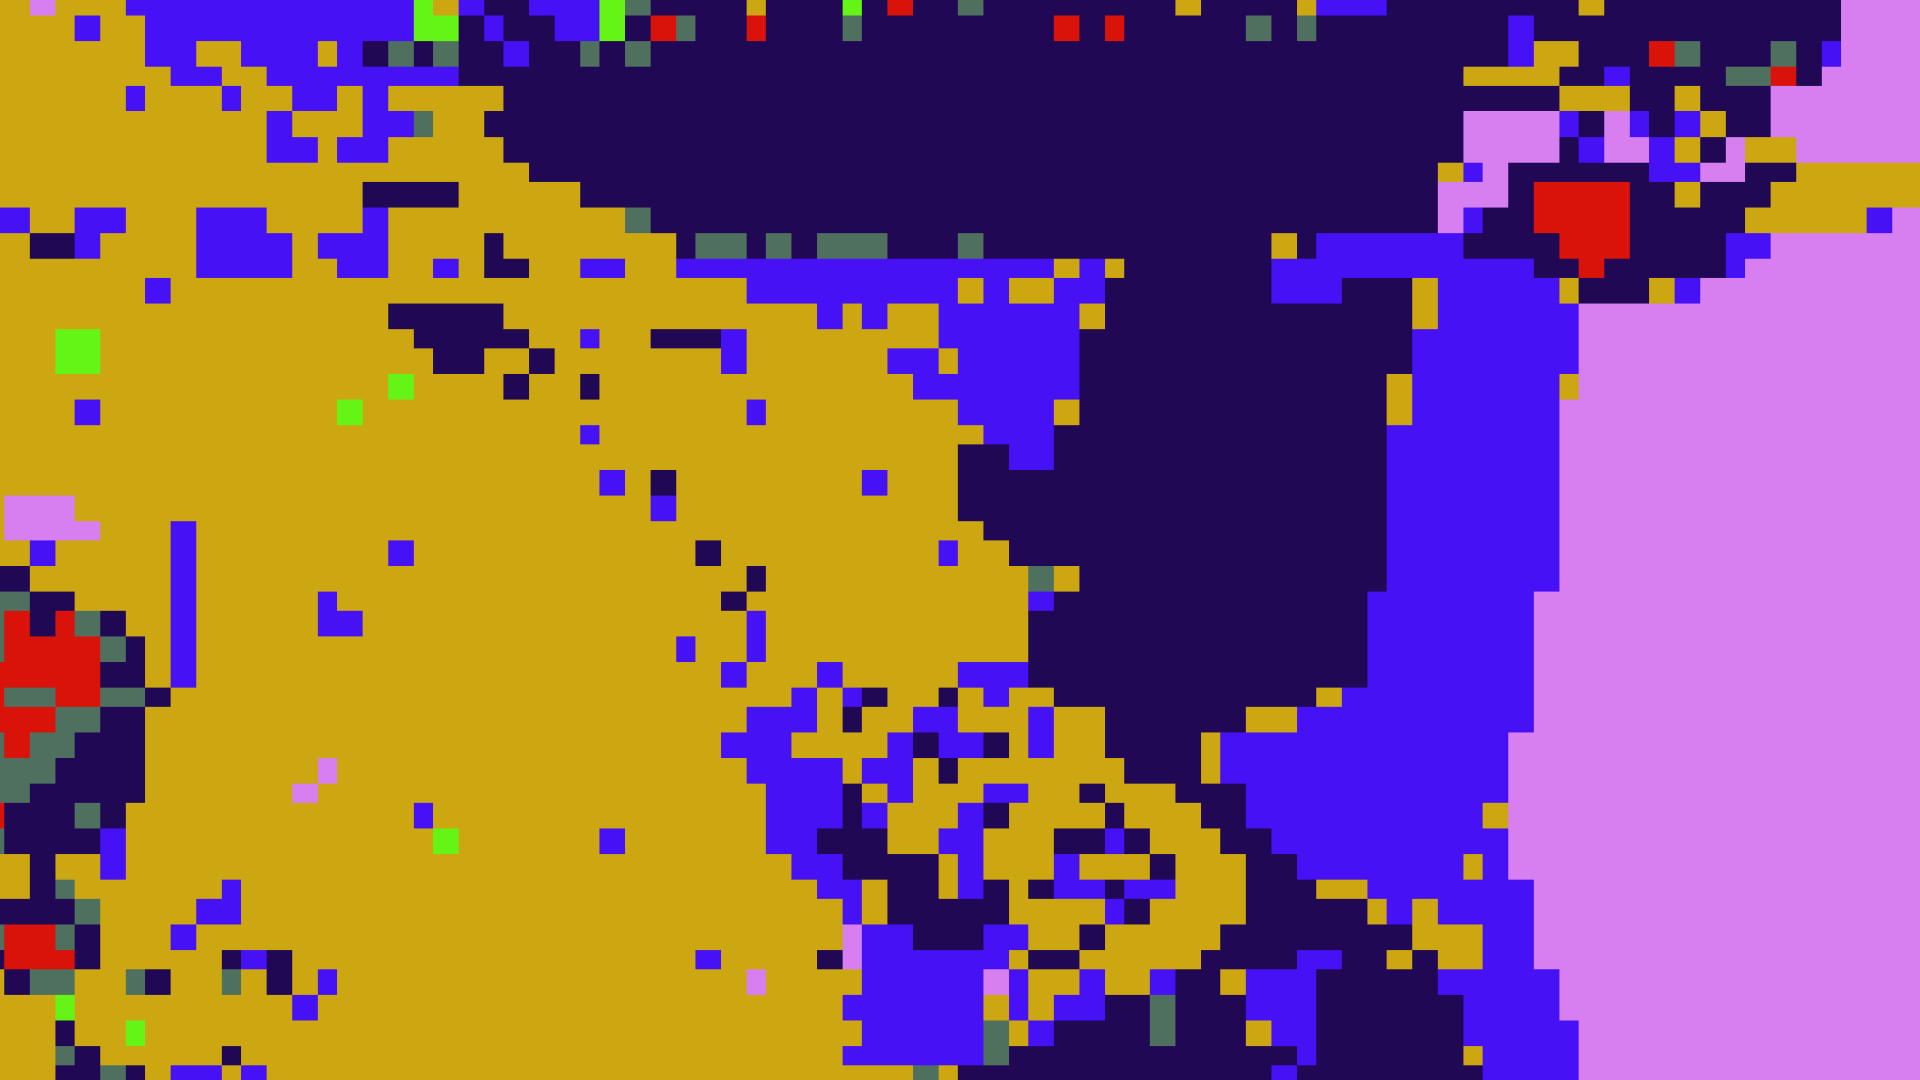
\includegraphics[width=.32\linewidth]{../images/areaUrbana/class}
		\caption{Área urbana}
	\end{figure}
	\begin{figure}[H]
		\centering
		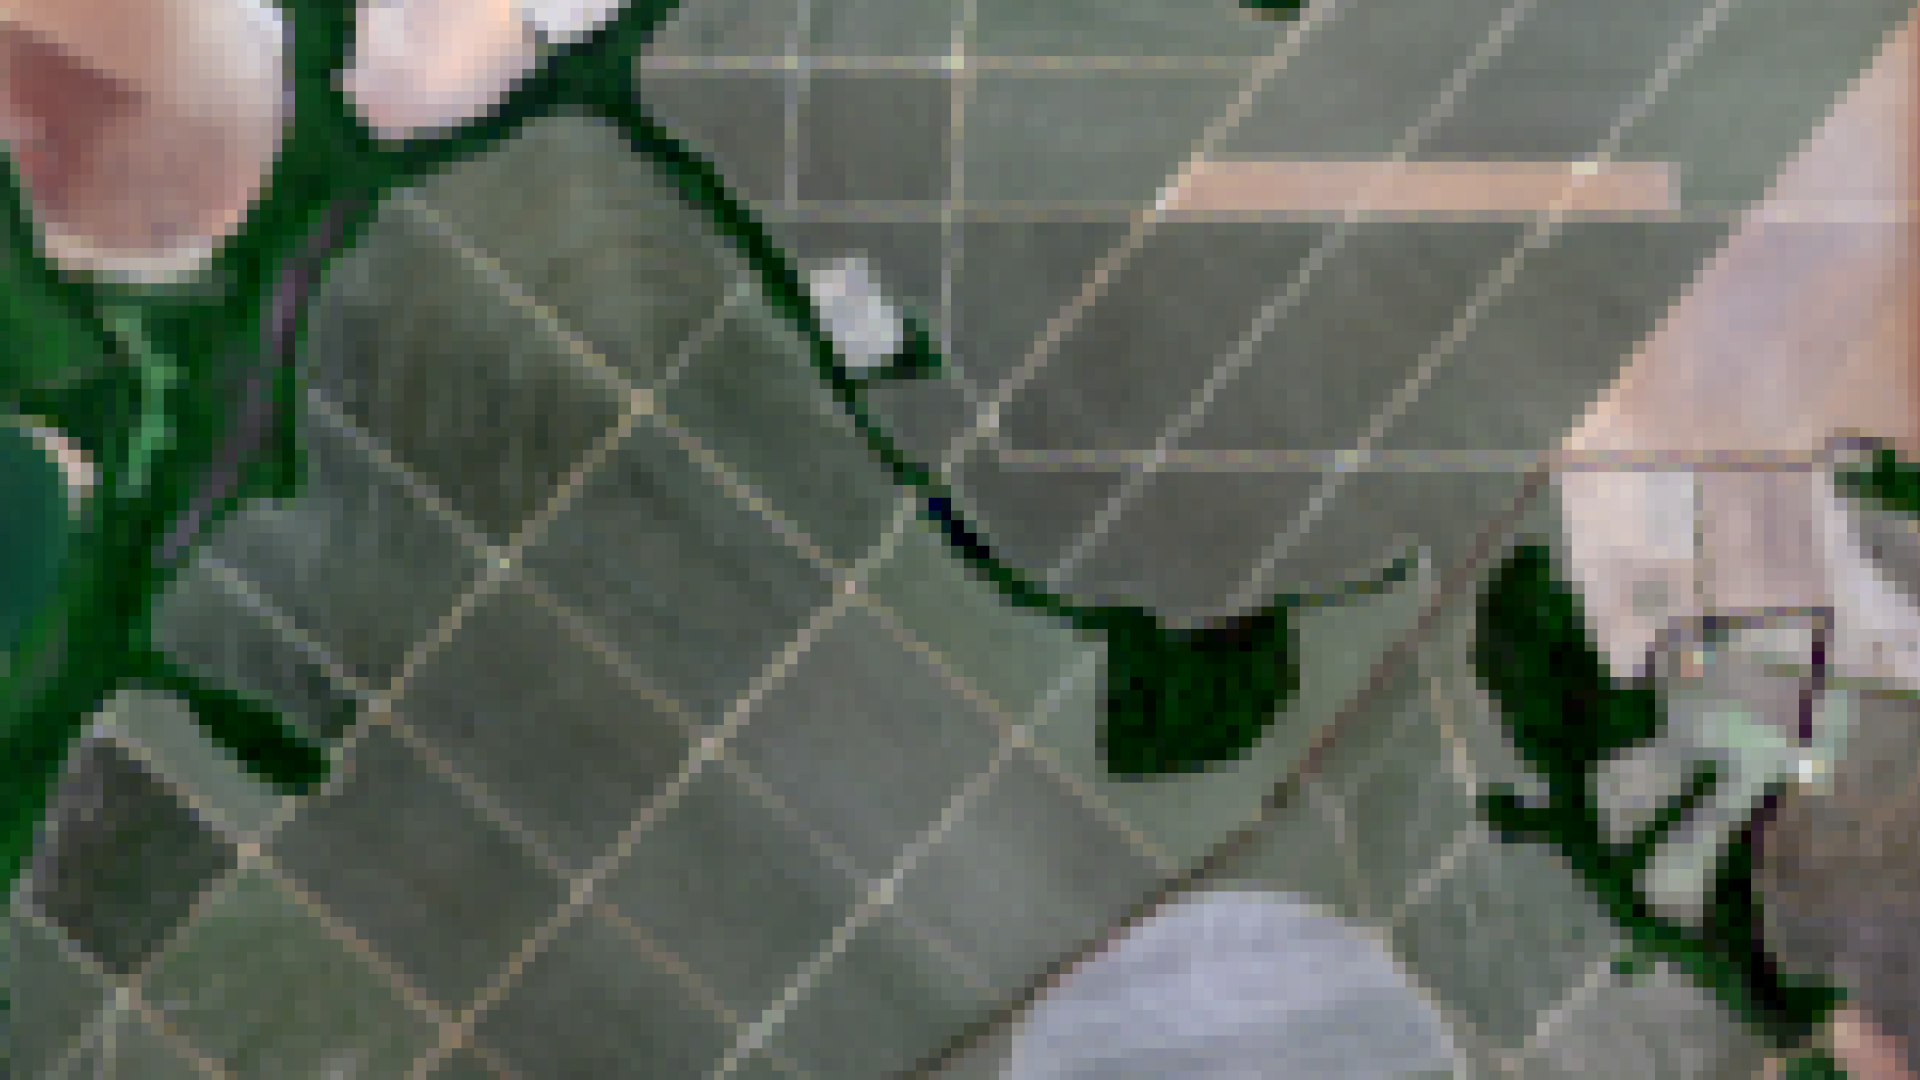
\includegraphics[width=.32\linewidth]{../images/florestaPlantada/432}
		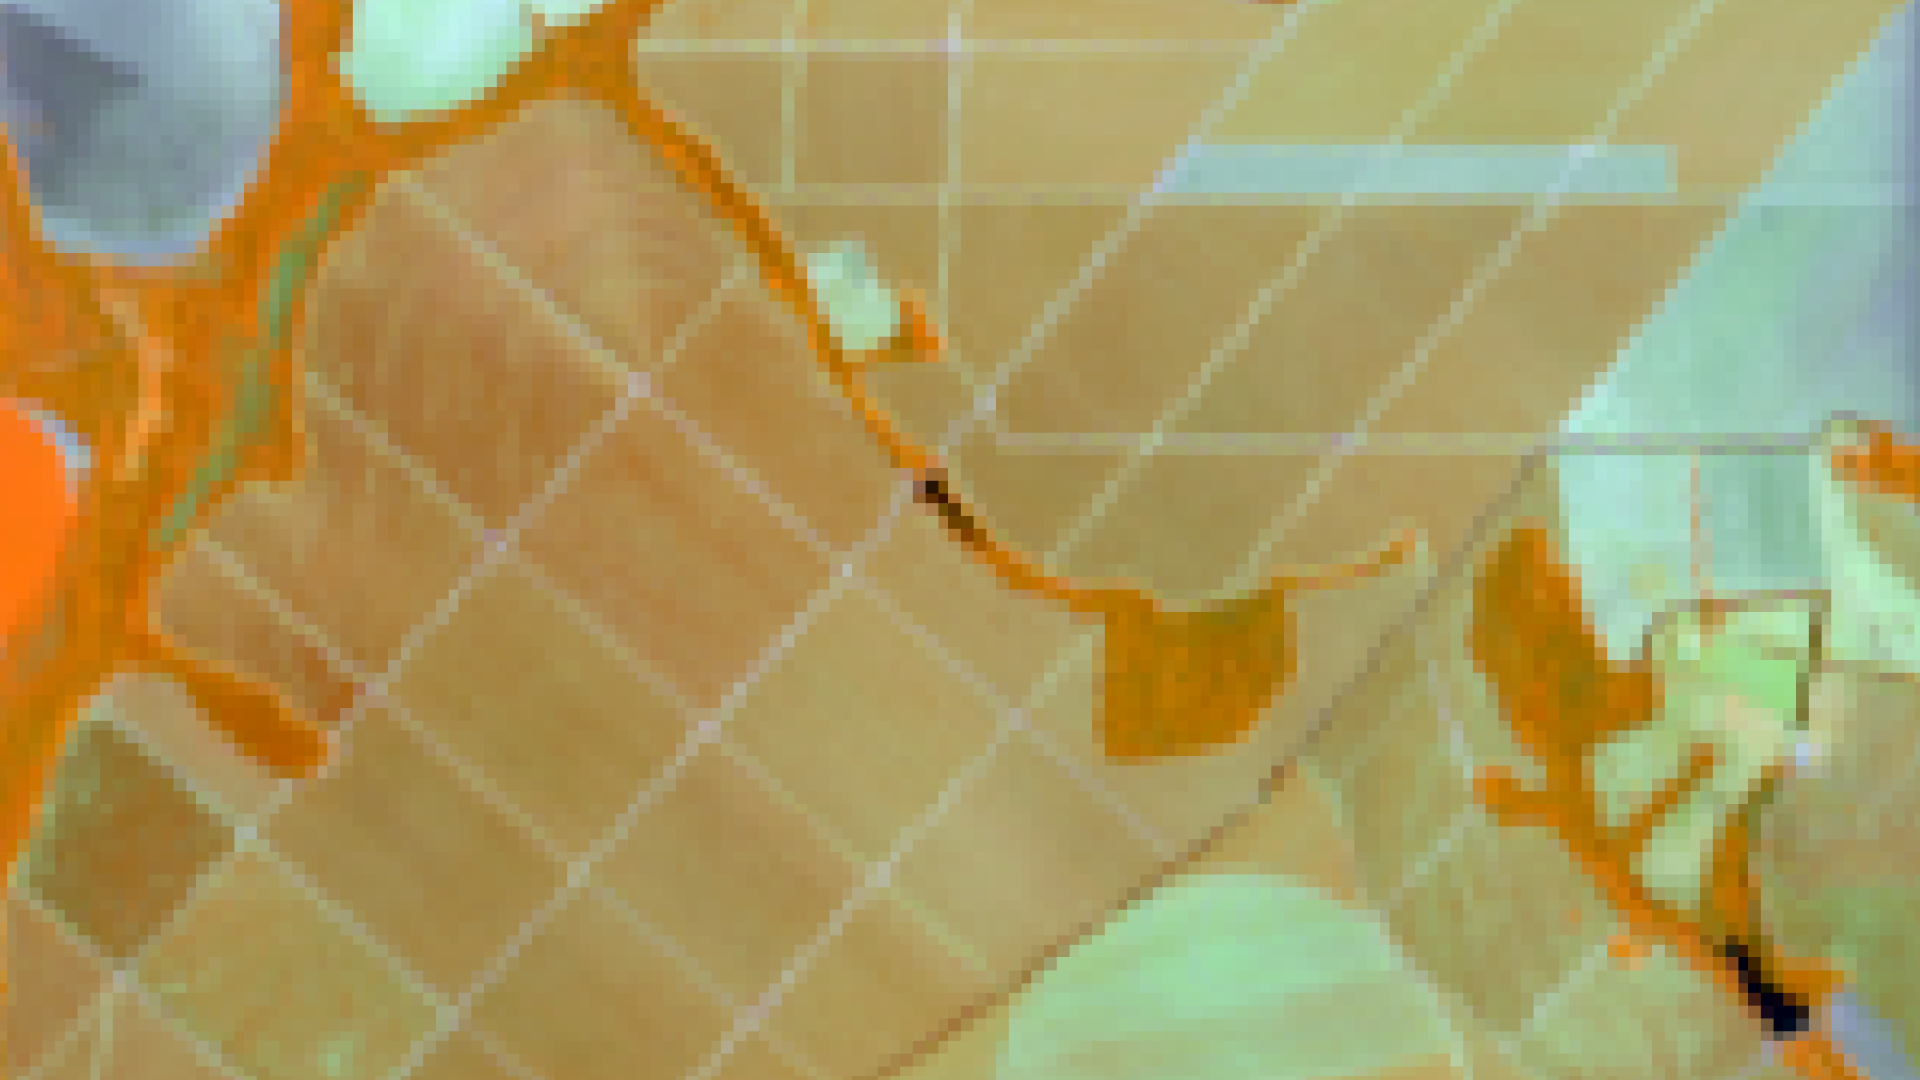
\includegraphics[width=.32\linewidth]{../images/florestaPlantada/564}
		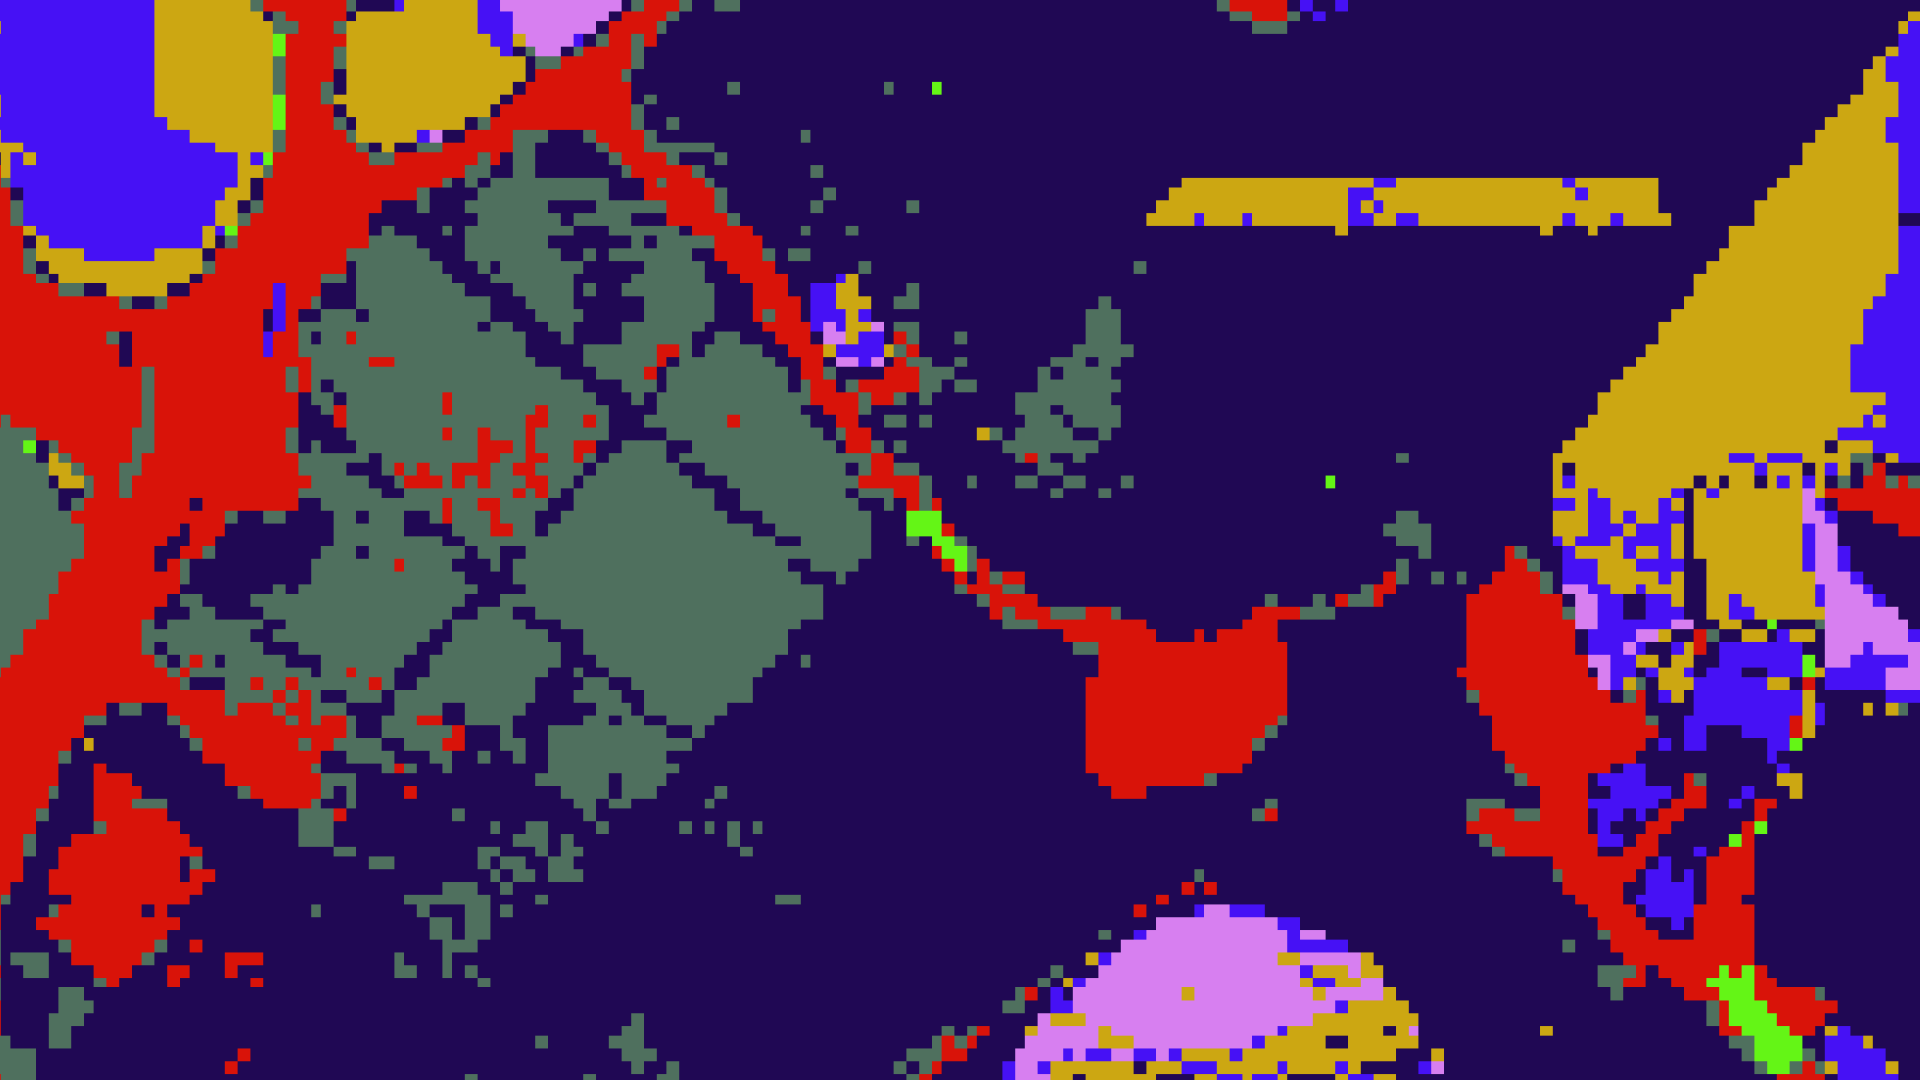
\includegraphics[width=.32\linewidth]{../images/florestaPlantada/class}
		\caption{Floresta plantada}
	\end{figure}
	\begin{figure}[H]
		\centering
		\includegraphics[width=.32\linewidth]{../images/vegetacaoNatural/432}
		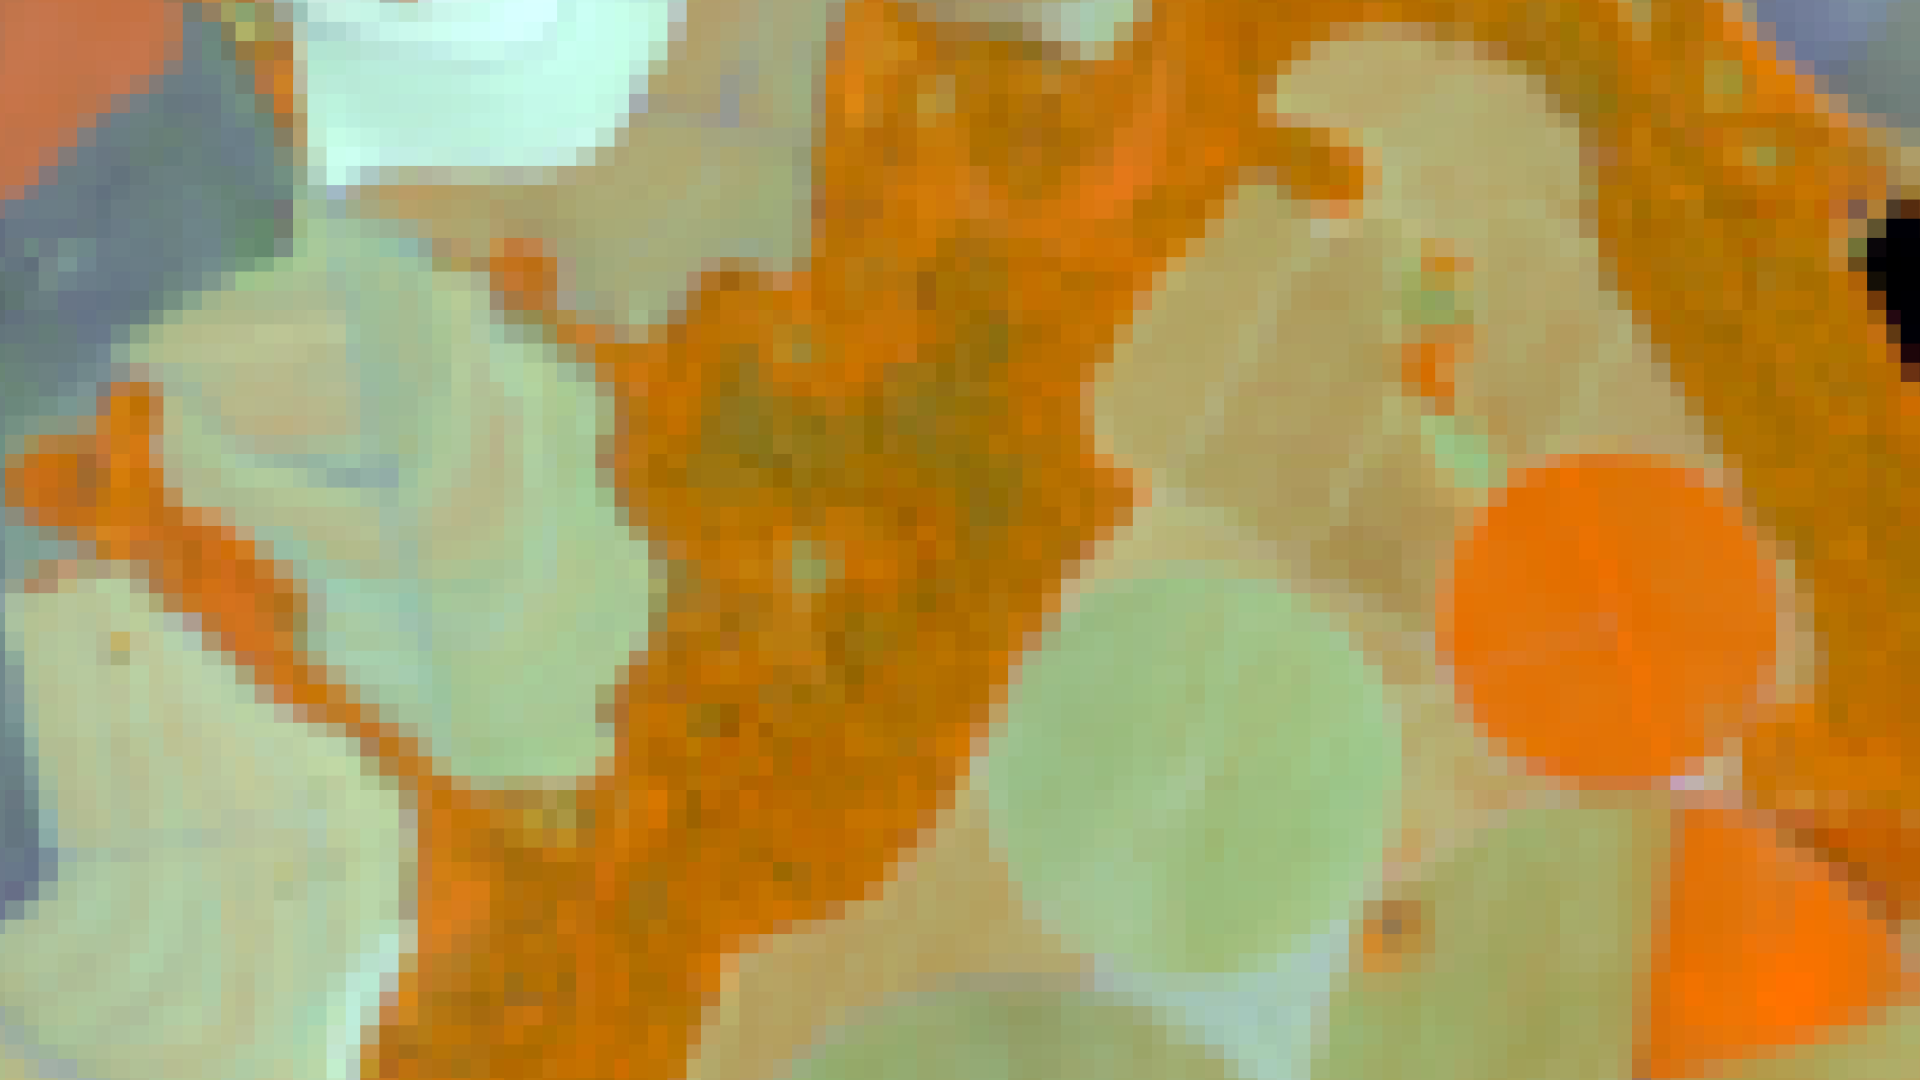
\includegraphics[width=.32\linewidth]{../images/vegetacaoNatural/564}
		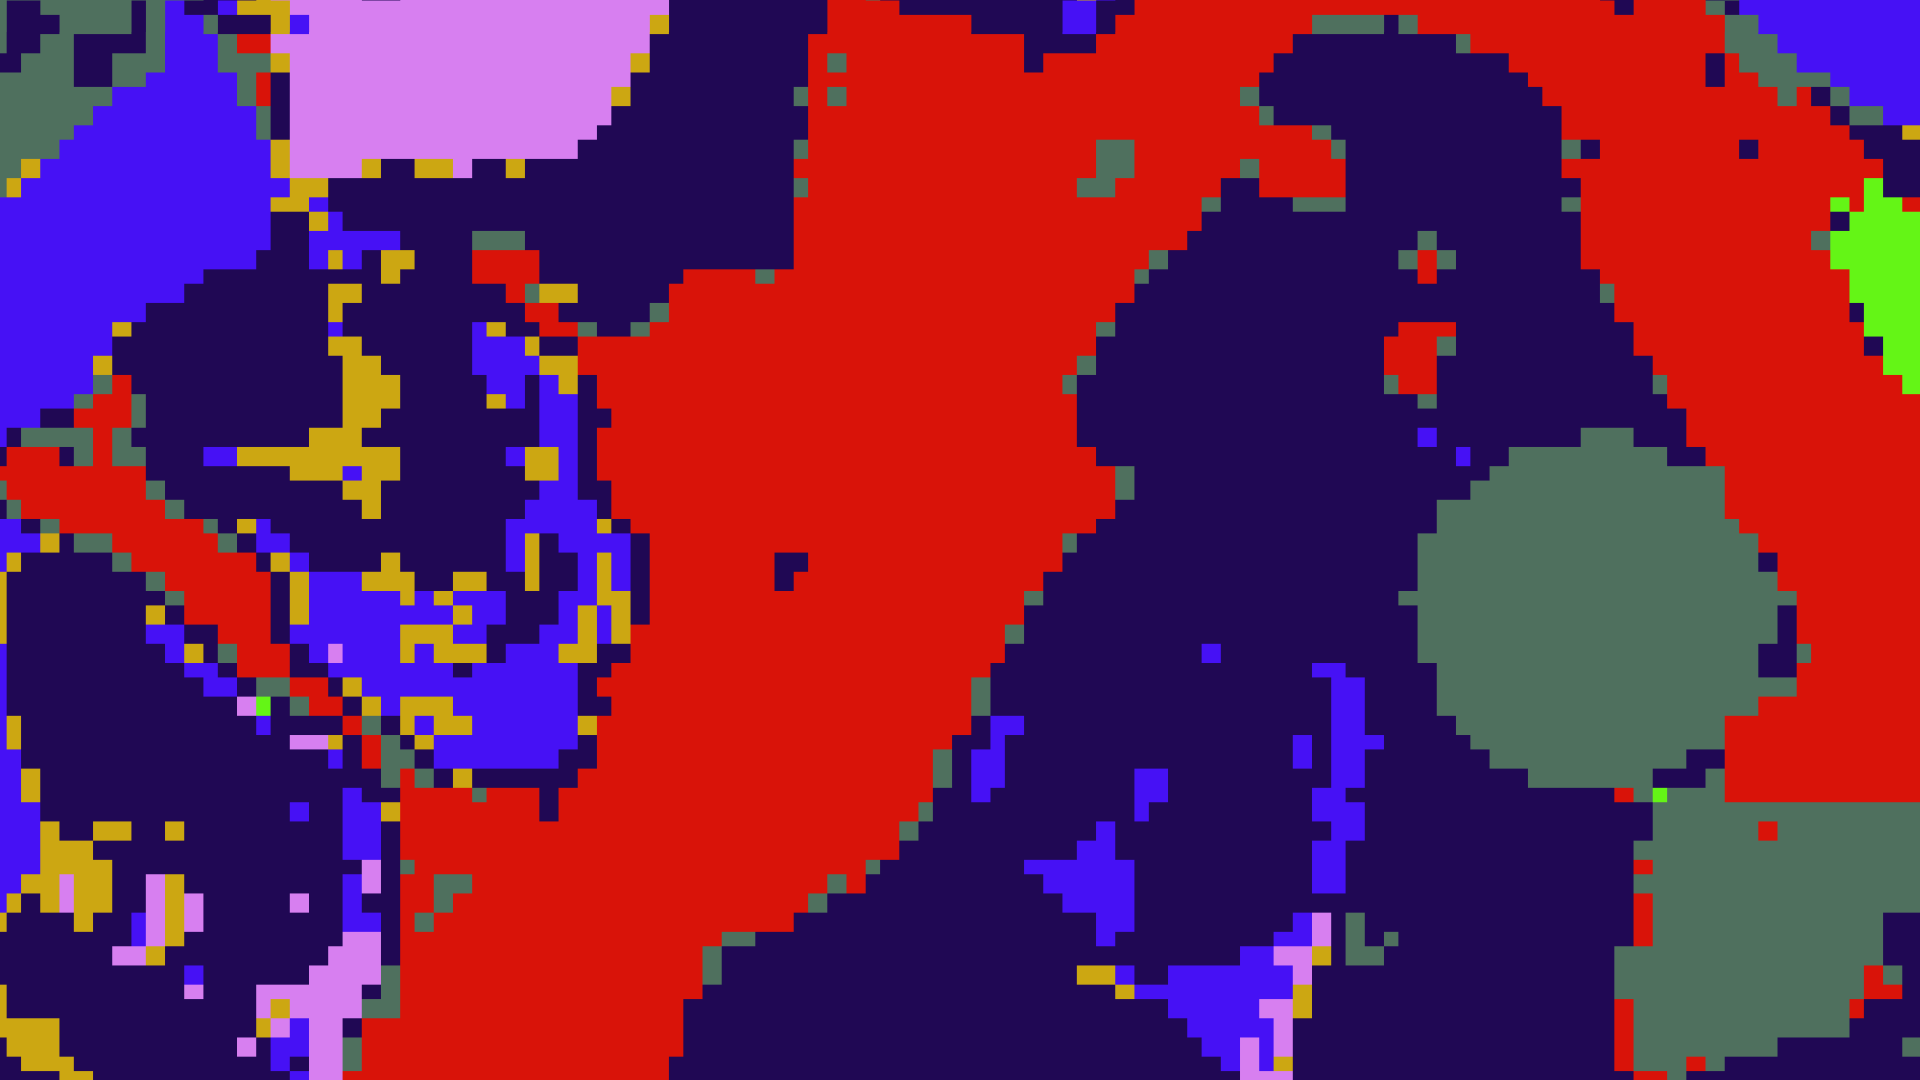
\includegraphics[width=.32\linewidth]{../images/vegetacaoNatural/class}
		\caption{Vegetação Natural}
	\end{figure}	
\end{document}